% Options for packages loaded elsewhere
\PassOptionsToPackage{unicode}{hyperref}
\PassOptionsToPackage{hyphens}{url}
%
\documentclass[
]{book}
\usepackage{amsmath,amssymb}
\usepackage{iftex}
\ifPDFTeX
  \usepackage[T1]{fontenc}
  \usepackage[utf8]{inputenc}
  \usepackage{textcomp} % provide euro and other symbols
\else % if luatex or xetex
  \usepackage{unicode-math} % this also loads fontspec
  \defaultfontfeatures{Scale=MatchLowercase}
  \defaultfontfeatures[\rmfamily]{Ligatures=TeX,Scale=1}
\fi
\usepackage{lmodern}
\ifPDFTeX\else
  % xetex/luatex font selection
\fi
% Use upquote if available, for straight quotes in verbatim environments
\IfFileExists{upquote.sty}{\usepackage{upquote}}{}
\IfFileExists{microtype.sty}{% use microtype if available
  \usepackage[]{microtype}
  \UseMicrotypeSet[protrusion]{basicmath} % disable protrusion for tt fonts
}{}
\makeatletter
\@ifundefined{KOMAClassName}{% if non-KOMA class
  \IfFileExists{parskip.sty}{%
    \usepackage{parskip}
  }{% else
    \setlength{\parindent}{0pt}
    \setlength{\parskip}{6pt plus 2pt minus 1pt}}
}{% if KOMA class
  \KOMAoptions{parskip=half}}
\makeatother
\usepackage{xcolor}
\usepackage{color}
\usepackage{fancyvrb}
\newcommand{\VerbBar}{|}
\newcommand{\VERB}{\Verb[commandchars=\\\{\}]}
\DefineVerbatimEnvironment{Highlighting}{Verbatim}{commandchars=\\\{\}}
% Add ',fontsize=\small' for more characters per line
\usepackage{framed}
\definecolor{shadecolor}{RGB}{248,248,248}
\newenvironment{Shaded}{\begin{snugshade}}{\end{snugshade}}
\newcommand{\AlertTok}[1]{\textcolor[rgb]{0.94,0.16,0.16}{#1}}
\newcommand{\AnnotationTok}[1]{\textcolor[rgb]{0.56,0.35,0.01}{\textbf{\textit{#1}}}}
\newcommand{\AttributeTok}[1]{\textcolor[rgb]{0.13,0.29,0.53}{#1}}
\newcommand{\BaseNTok}[1]{\textcolor[rgb]{0.00,0.00,0.81}{#1}}
\newcommand{\BuiltInTok}[1]{#1}
\newcommand{\CharTok}[1]{\textcolor[rgb]{0.31,0.60,0.02}{#1}}
\newcommand{\CommentTok}[1]{\textcolor[rgb]{0.56,0.35,0.01}{\textit{#1}}}
\newcommand{\CommentVarTok}[1]{\textcolor[rgb]{0.56,0.35,0.01}{\textbf{\textit{#1}}}}
\newcommand{\ConstantTok}[1]{\textcolor[rgb]{0.56,0.35,0.01}{#1}}
\newcommand{\ControlFlowTok}[1]{\textcolor[rgb]{0.13,0.29,0.53}{\textbf{#1}}}
\newcommand{\DataTypeTok}[1]{\textcolor[rgb]{0.13,0.29,0.53}{#1}}
\newcommand{\DecValTok}[1]{\textcolor[rgb]{0.00,0.00,0.81}{#1}}
\newcommand{\DocumentationTok}[1]{\textcolor[rgb]{0.56,0.35,0.01}{\textbf{\textit{#1}}}}
\newcommand{\ErrorTok}[1]{\textcolor[rgb]{0.64,0.00,0.00}{\textbf{#1}}}
\newcommand{\ExtensionTok}[1]{#1}
\newcommand{\FloatTok}[1]{\textcolor[rgb]{0.00,0.00,0.81}{#1}}
\newcommand{\FunctionTok}[1]{\textcolor[rgb]{0.13,0.29,0.53}{\textbf{#1}}}
\newcommand{\ImportTok}[1]{#1}
\newcommand{\InformationTok}[1]{\textcolor[rgb]{0.56,0.35,0.01}{\textbf{\textit{#1}}}}
\newcommand{\KeywordTok}[1]{\textcolor[rgb]{0.13,0.29,0.53}{\textbf{#1}}}
\newcommand{\NormalTok}[1]{#1}
\newcommand{\OperatorTok}[1]{\textcolor[rgb]{0.81,0.36,0.00}{\textbf{#1}}}
\newcommand{\OtherTok}[1]{\textcolor[rgb]{0.56,0.35,0.01}{#1}}
\newcommand{\PreprocessorTok}[1]{\textcolor[rgb]{0.56,0.35,0.01}{\textit{#1}}}
\newcommand{\RegionMarkerTok}[1]{#1}
\newcommand{\SpecialCharTok}[1]{\textcolor[rgb]{0.81,0.36,0.00}{\textbf{#1}}}
\newcommand{\SpecialStringTok}[1]{\textcolor[rgb]{0.31,0.60,0.02}{#1}}
\newcommand{\StringTok}[1]{\textcolor[rgb]{0.31,0.60,0.02}{#1}}
\newcommand{\VariableTok}[1]{\textcolor[rgb]{0.00,0.00,0.00}{#1}}
\newcommand{\VerbatimStringTok}[1]{\textcolor[rgb]{0.31,0.60,0.02}{#1}}
\newcommand{\WarningTok}[1]{\textcolor[rgb]{0.56,0.35,0.01}{\textbf{\textit{#1}}}}
\usepackage{longtable,booktabs,array}
\usepackage{calc} % for calculating minipage widths
% Correct order of tables after \paragraph or \subparagraph
\usepackage{etoolbox}
\makeatletter
\patchcmd\longtable{\par}{\if@noskipsec\mbox{}\fi\par}{}{}
\makeatother
% Allow footnotes in longtable head/foot
\IfFileExists{footnotehyper.sty}{\usepackage{footnotehyper}}{\usepackage{footnote}}
\makesavenoteenv{longtable}
\usepackage{graphicx}
\makeatletter
\def\maxwidth{\ifdim\Gin@nat@width>\linewidth\linewidth\else\Gin@nat@width\fi}
\def\maxheight{\ifdim\Gin@nat@height>\textheight\textheight\else\Gin@nat@height\fi}
\makeatother
% Scale images if necessary, so that they will not overflow the page
% margins by default, and it is still possible to overwrite the defaults
% using explicit options in \includegraphics[width, height, ...]{}
\setkeys{Gin}{width=\maxwidth,height=\maxheight,keepaspectratio}
% Set default figure placement to htbp
\makeatletter
\def\fps@figure{htbp}
\makeatother
\setlength{\emergencystretch}{3em} % prevent overfull lines
\providecommand{\tightlist}{%
  \setlength{\itemsep}{0pt}\setlength{\parskip}{0pt}}
\setcounter{secnumdepth}{5}
\usepackage{booktabs}
\ifLuaTeX
  \usepackage{selnolig}  % disable illegal ligatures
\fi
\usepackage[]{natbib}
\bibliographystyle{apalike}
\usepackage{bookmark}
\IfFileExists{xurl.sty}{\usepackage{xurl}}{} % add URL line breaks if available
\urlstyle{same}
\hypersetup{
  pdftitle={R Development Guide},
  pdfauthor={R Contribution Working Group},
  hidelinks,
  pdfcreator={LaTeX via pandoc}}

\title{R Development Guide}
\author{R Contribution Working Group}
\date{2024-07-19}

\begin{document}
\maketitle

{
\setcounter{tocdepth}{1}
\tableofcontents
}
\chapter*{}\label{section}
\addcontentsline{toc}{chapter}{}

\begin{figure}
\centering

\includegraphics[width=5.20833in,height=4.16667in]{img/Rlogo.png}
\caption{R Logo}
\end{figure}

\chapter*{Acknowledgement}\label{acknowledgement}
\addcontentsline{toc}{chapter}{Acknowledgement}

This guide draws on documentation and articles written by the R Core Team. The first version of the guide was heavily influenced by the \href{https://devguide.python.org/}{Python Developer's Guide}.

Initial chapters of the guide were developed by Saranjeet Kaur Bhogal, in a project funded by the R Foundation, mentored by Heather Turner and Michael Lawrence. This initial version was upgraded in a \href{https://github.com/rstats-gsod/gsod2022/wiki/GSOD-2022-Proposal}{Google Season of Docs 2022} project with Saranjeet Kaur Bhogal and Lluís Revilla Sancho working as technical writers managed by Nicolas Bennett and overseen by a \href{https://github.com/rstats-gsod/gsod2022/wiki/GSOD-2022-Proposal\#steering-committee}{Steering Committee} including representatives from R Core and the wider R community.

This guide has benefited and continues to benefit from varied contributions by several \href{https://github.com/r-devel/rdevguide\#contributors-}{contributors}.

\href{https://creativecommons.org/licenses/by/4.0/}{
\includegraphics{img/ccby.png}}

This project is licensed under a \href{https://creativecommons.org/licenses/by/4.0/}{Creative Commons Attribution 4.0 International (CC BY 4.0)}. Some pages may contain materials that are subject to copyright, in which case you will see the copyright notice.

\chapter{Introduction}\label{introduction}

This guide is a comprehensive resource for contributing to base R\footnote{The \href{https://cran.r-project.org/doc/FAQ/R-FAQ.html\#Add_002don-packages-in-R}{set of packages} in the base R distribution that are maintained by the R Core Team.} -- for both new and experienced contributors. It is maintained by the \href{/working-group}{R Contribution Working Group}. We welcome your contributions to base R!

\section{Overview of different ways of contributing to the base R Project}\label{overview-of-different-ways-of-contributing-to-the-base-r-project}

Contributions to base R are possible in a number of different ways. Some of them are listed below:

\begin{enumerate}
\def\labelenumi{\arabic{enumi}.}
\tightlist
\item
  Contributing to bug fixing: Refer \hyperref[BugTrack]{Bug Tracking} and \hyperref[ReviewBugs]{Reviewing Bugs}.
\item
  Contributing to translations: Refer \hyperref[]{Translations}.
\item
  Testing R before release: Refer \hyperref[TestRVer]{Testing Pre-release R Versions}.
\end{enumerate}

\section{Quick start to the guide}\label{quick-start-to-the-guide}

The guide is intended as a comprehensive resource for contributing to base R. The following chapter outline provides an overview with links to sections for getting started with contributing.

\begin{enumerate}
\def\labelenumi{\arabic{enumi}.}
\tightlist
\item
  The \hyperref[GetStart]{Getting Started} covers the instructions on how to install R on the major operating systems (Windows, Linux and macOS), as well as the tools required to build R and R packages from source.
\end{enumerate}

\begin{enumerate}
\def\labelenumi{\arabic{enumi}.}
\setcounter{enumi}{1}
\item
  The \hyperref[BugTrack]{Bug Tracking} and the \hyperref[ReviewBugs]{Reviewing Bugs} chapters discuss how to find bugs in R and how to review bug reports that are submitted to Bugzilla.
\item
  The \hyperref[FindSource]{Finding the Source} chapter provides an overview of the R codebase and helps with finding source code of base functions written in R and/or C.
\item
  The \hyperref[FixBug]{Lifecycle of a Patch} chapter discusses how to create a patch to propose a bug fix.
\item
  The \hyperref[Doc]{Documenting R} chapter describes the format and style guide for help files in R, how to report and review issues in the existing documentation and how to propose changes.
\item
  How to test pre-release versions of R is discussed in the chapter on \hyperref[TestRVer]{Testing Pre-release R Versions}.
\item
  The \hyperref[CoreDev]{R Core Developers} chapter contains a list of the former and current members of the R Core team who have write access to the R source.
\item
  For more information on how to engage with to community and ask for help, refer to the \hyperref[WhereToGetHelp]{Where to Get Help} chapter.
\item
  To keep up with the developments in R refer to some of the resources available in the \hyperref[News]{News and Announcements}
\item
  Resources and tools that may be relevant for R developers are available in the \hyperref[DevTools]{Developer Tools} chapter.
\end{enumerate}

\section{How to contribute to this guide itself?}\label{how-to-contribute-to-this-guide}

This guide is built using bookdown which makes editing it easier, provided you have a GitHub account (sign-up at \href{https://github.com/}{github.com}). After you log-in to GitHub, click on the `Edit' icon highlighted with a red ellipse in the image below. This will take you to an editable version of the the source R Markdown file that generated the page you are on:

\begin{figure}
\centering

\includegraphics{img/edit_icon.png}
\caption{Screenshot of the toolbar in the HTML version of the guide, with the Edit button (pencil and paper icon) circled in red.}
\end{figure}

Use the \href{https://github.com/r-devel/rdevguide/issues}{issue tracker} to raise an issue about the guide's content or to make a feature request.

Maintainers and contributors are requested to follow this project's \href{https://github.com/r-devel/rdevguide/blob/main/CONDUCT.md}{code of conduct}.

\chapter{R Patched and Development Versions}\label{GetStart}

These instructions cover how to install R from source or from binaries.
Contributors will typically need to work with the patched or development versions of R.
This chapter describes where the source code for these versions can be found and how to install these versions from the source or the binary builds (where available).
The tools required to build R and R packages are also discussed.
For the most up to date and complete instructions you can check the \href{https://cran.r-project.org/doc/manuals/r-devel/R-admin.html}{R installation and administration manual} .

\section{The R source code}\label{the-r-source-code}

R uses \href{https://subversion.apache.org/}{svn} as a version control tool hosted at \url{https://svn.r-project.org/R/} and uses a `major.minor.patchlevel' version numbering scheme\footnote{Also known as \href{https://en.wikipedia.org/wiki/Software_versioning\#Semantic_versioning}{semantic versioning}}.

There are three releases of R available to install:

\begin{itemize}
\item
  The latest official release (\texttt{r-release}), either major version x.0.0 or minor version x.y.0, for example: 3.0.0 or 3.2.0
\item
  The patched release (\texttt{r-patched}), for example 3.0.1 or 3.2.1 and
\item
  The development release (\texttt{r-devel}) : continually developed version moving from r-release to next major/minor version (x + 1).0.0 or x.(y + 1).0 a few weeks before release (at the start of the ``GRAND FEATURE FREEZE'').
\end{itemize}

The source code of released versions of R can be found at \href{https://svn.r-project.org/R/tags/}{R/tags}, the patched versions are at \href{https://svn.r-project.org/R/branches/}{R/branch}.

The \texttt{r-devel} at \href{https://svn.r-project.org/R/trunk}{R/trunk} is the next minor or eventual major release development version of R.
Bug fixes and new features are introduced in \texttt{r-devel} first.
If the change meets the \href{https://developer.r-project.org/devel-guidelines.txt}{development guidelines} R Core will also make the change in \texttt{r-patched}.

\section{Prerequisites}\label{prerequisites}

To install from the source code you will need the source code and the dependencies of R.

If you need to install svn you can use your distribution's package manager to install it.

\subsection{Ubuntu}\label{ubuntu}

In Ubuntu you can use this command to find all the dependencies of R:

\begin{Shaded}
\begin{Highlighting}[]
\ExtensionTok{apt{-}rdepends} \AttributeTok{{-}{-}build{-}depends} \AttributeTok{{-}{-}follow}\OperatorTok{=}\NormalTok{DEPENDS r{-}base{-}dev }\KeywordTok{|} \FunctionTok{grep} \StringTok{" B"} \KeywordTok{|} \FunctionTok{sed} \AttributeTok{{-}e} \StringTok{"s/  Build{-}Depends: //"}
\end{Highlighting}
\end{Shaded}

It might require installation of apt-rdepends which can be done from default repositories via \texttt{sudo\ apt-get\ install\ apt-rdepends}.

To install all the R dependencies you can use:

\begin{Shaded}
\begin{Highlighting}[]
\FunctionTok{sudo}\NormalTok{ apt{-}get build{-}dep r{-}base{-}dev}
\end{Highlighting}
\end{Shaded}

\subsection{Fedora}\label{fedora}

In Fedora you can use this command to find all the dependencies of R:

\begin{Shaded}
\begin{Highlighting}[]
\ExtensionTok{dnf}\NormalTok{ rq }\AttributeTok{{-}q} \AttributeTok{{-}{-}repo}\OperatorTok{=}\NormalTok{fedora{-}source }\AttributeTok{{-}{-}requires}\NormalTok{ R }
\end{Highlighting}
\end{Shaded}

You will also need the rsync package to download the recommended packages.

To install them you can use:

\begin{Shaded}
\begin{Highlighting}[]
\ExtensionTok{dnf}\NormalTok{ install }\StringTok{\textquotesingle{}dnf{-}command(builddep)\textquotesingle{}}
\ExtensionTok{dnf}\NormalTok{ install rsync}
\ExtensionTok{dnf}\NormalTok{ builddep R}
\end{Highlighting}
\end{Shaded}

\section{Building R}\label{building-r}

\subsection{Linux}\label{linux}

Here are the basic steps intended as a checklist.
For complete instructions please see the section in \href{https://cran.r-project.org/doc/manuals/r-devel/R-admin.html\#Installing-R-under-Unix_002dalikes}{R-admin}.

\begin{enumerate}
\def\labelenumi{\arabic{enumi}.}
\setcounter{enumi}{-1}
\item
  Retrieve R source code via into \texttt{TOP\_SRCDIR}, note that we retrieve the \texttt{r-devel} source code:

\begin{Shaded}
\begin{Highlighting}[]
\BuiltInTok{export} \VariableTok{TOP\_SRCDIR}\OperatorTok{=}\StringTok{"}\VariableTok{$HOME}\StringTok{/Downloads/R"}
\FunctionTok{svn}\NormalTok{ checkout https://svn.r{-}project.org/R/trunk/ }\StringTok{"}\VariableTok{$TOP\_SRCDIR}\StringTok{"}
\end{Highlighting}
\end{Shaded}
\item
  Download the latest recommended packages\footnote{Recommended packages are not in the subversion repository.}:

\begin{Shaded}
\begin{Highlighting}[]
\StringTok{"}\VariableTok{$TOP\_SRCDIR}\StringTok{/tools/rsync{-}recommended"}
\end{Highlighting}
\end{Shaded}
\item
  Create the build directory in the \texttt{BUILDDIR}:

\begin{Shaded}
\begin{Highlighting}[]
\BuiltInTok{export} \VariableTok{BUILDDIR}\OperatorTok{=}\StringTok{"}\VariableTok{$HOME}\StringTok{/bin/R"}
\FunctionTok{mkdir} \AttributeTok{{-}p} \StringTok{"}\VariableTok{$BUILDDIR}\StringTok{"}
\BuiltInTok{cd} \StringTok{"}\VariableTok{$BUILDDIR}\StringTok{"}
\end{Highlighting}
\end{Shaded}
\item
  Configure the R installation (with \texttt{-\/-enable-R-shlib} so that RStudio IDE can use it):

\begin{Shaded}
\begin{Highlighting}[]
\StringTok{"}\VariableTok{$TOP\_SRCDIR}\StringTok{/configure"} \AttributeTok{{-}{-}enable{-}R{-}shlib}
\end{Highlighting}
\end{Shaded}
\item
  Build R :

\begin{Shaded}
\begin{Highlighting}[]
\FunctionTok{make}
\end{Highlighting}
\end{Shaded}
\item
  Check that R works as expected:

\begin{Shaded}
\begin{Highlighting}[]
\FunctionTok{make}\NormalTok{ check}
\end{Highlighting}
\end{Shaded}

  There are other checks you can run:

\begin{Shaded}
\begin{Highlighting}[]
\FunctionTok{make}\NormalTok{ check{-}devel}
\FunctionTok{make}\NormalTok{ check{-}recommended}
\end{Highlighting}
\end{Shaded}
\end{enumerate}

If we don't want to build R in a different directory than the source code we can simply use:

\begin{Shaded}
\begin{Highlighting}[]
\BuiltInTok{cd} \StringTok{"}\VariableTok{$TOP\_SRCDIR}\StringTok{"}
\FunctionTok{svn}\NormalTok{ update}
\ExtensionTok{tools/rsync{-}recommended}
\StringTok{"}\VariableTok{$TOP\_SRCDIR}\StringTok{/configure"}  \AttributeTok{{-}{-}enable{-}R{-}shlib}
\FunctionTok{make} 
\FunctionTok{make}\NormalTok{ check}
\end{Highlighting}
\end{Shaded}

Once you successfully built R from source you can modify the R source code to fix an issue: Prepare a patch (See \href{https://www.r-project.org/bugs.html\#how-to-submit-patches}{this guide}) and after checking that R works as intended (\texttt{make\ check-devel}) submit the patch for consideration by R Core.
(See the \hyperref[FixBug]{lifecycle of a patch} chapter).

To use the \texttt{r-devel} version in RStudio, you can do the following:

\begin{Shaded}
\begin{Highlighting}[]
\BuiltInTok{export} \VariableTok{RSTUDIO\_WHICH\_R}\OperatorTok{=}\StringTok{"}\VariableTok{$BUILDDIR}\StringTok{/bin/R"}
\BuiltInTok{cd} \StringTok{"}\VariableTok{$TOP\_SRCDIR}\StringTok{"}
\ExtensionTok{rstudio}
\end{Highlighting}
\end{Shaded}

\subsection{Windows}\label{windows}

\subsubsection{Binaries}\label{binaries}

The binary builds of R for Windows can be downloaded and installed from \href{https://cran.r-project.org/bin/windows/base/}{here}.
Along with the link to the latest stable release, this page also contains links to the binary builds of \texttt{r-patched} and \texttt{r-devel}.

\begin{enumerate}
\def\labelenumi{\arabic{enumi}.}
\item
  Click on the download links to download an executable installer.
\item
  Select the language while installing, read the GNU general public license information, and select the destination location to start the installation.
  You will be prompted to select components at this stage: \texttt{User\ installation}, \texttt{64-bit\ User\ installation}, or \texttt{Custom\ installation}.
  The default option may be chosen for the questions from this step onwards to complete the installation.
\end{enumerate}

Daily binaries for \texttt{r-devel} are made available for \href{https://cran.r-project.org/bin/windows/base/rdevel.html}{download and installation}.

\subsubsection{From source}\label{windowsSource}

Before installing R from source, some additional programs are needed, as per the \href{https://cran.r-project.org/bin/windows/base/howto-R-4.2.html}{latest documentation}:

\begin{enumerate}
\def\labelenumi{\arabic{enumi}.}
\item
  \href{https://cran.r-project.org/bin/windows/Rtools/}{Rtools} is the suggested toolchain bundle for building R base and R packages containing compiled code on Windows.
  The latest \href{https://cran.r-project.org/bin/windows/Rtools/rtools44/rtools.html}{version of Rtools} can be installed using the \href{https://cran.r-project.org/bin/windows/Rtools/rtools44/files/}{Rtools installer rtools44-XXXX-XXX.exe}.
\item
  A LaTeX compiler is needed to install and build R, check packages and build manuals.
  On CRAN, MiKTeX is used, which can be downloaded from \url{https://miktex.org}.
  Once installed open MiKTeX via the Windows start menu.
  It might ask to check for updates and more importantly, to make it available in PATH. You can accept both.
\item
  Open the Rtools43 terminal to update and install subversion:

\begin{Shaded}
\begin{Highlighting}[]
\ExtensionTok{pacman} \AttributeTok{{-}Syuu}
\ExtensionTok{pacman} \AttributeTok{{-}Sy}\NormalTok{ wget subversion}
\end{Highlighting}
\end{Shaded}
\item
  Retrieve the latest source code via subversion:

\begin{Shaded}
\begin{Highlighting}[]
\BuiltInTok{export} \VariableTok{TOP\_SRCDIR}\OperatorTok{=}\StringTok{"}\VariableTok{$HOME}\StringTok{/Downloads/R"}
\FunctionTok{svn}\NormalTok{ checkout https://svn.r{-}project.org/R/trunk/ }\StringTok{"}\VariableTok{$TOP\_SRCDIR}\StringTok{"}
\end{Highlighting}
\end{Shaded}

  If you already have the repository available you can update as:

\begin{Shaded}
\begin{Highlighting}[]
\BuiltInTok{cd} \VariableTok{$TOP\_SRCDIR}
\FunctionTok{svn}\NormalTok{ update}
\end{Highlighting}
\end{Shaded}

  You can also use a SVN client such as TortoiseSVN (\url{https://tortoisesvn.net/}, command line tool, and Windows Explorer integration) or SlikSVN (\url{https://sliksvn.com/download/}, just the command line tool) so that it can be also found by other tools.
\item
  Download the latest tcl/tk and unzip it in \texttt{\$TOP\_SRCDIR}:

\begin{Shaded}
\begin{Highlighting}[]
\BuiltInTok{cd} \StringTok{"}\VariableTok{$TOP\_SRCDIR}\StringTok{"}
\FunctionTok{wget} \AttributeTok{{-}np} \AttributeTok{{-}nd} \AttributeTok{{-}r} \AttributeTok{{-}l1} \AttributeTok{{-}A} \StringTok{\textquotesingle{}tcltk{-}*.zip\textquotesingle{}}\NormalTok{ https://cran.r{-}project.org/bin/windows/Rtools/rtools43/files/}
\FunctionTok{unzip} \StringTok{"tcltk{-}*.zip"}
\end{Highlighting}
\end{Shaded}
\item
  Add gcc, MiKTeX and tar to the PATH and set one tar option:

\begin{Shaded}
\begin{Highlighting}[]
\BuiltInTok{export} \VariableTok{PATH}\OperatorTok{=}\StringTok{"/x86\_64{-}w64{-}mingw32.static.posix/bin:}\VariableTok{$PATH}\StringTok{"}
\BuiltInTok{export} \VariableTok{PATH}\OperatorTok{=}\StringTok{"/c/Program Files/MiKTeX/miktex/bin/x64:}\VariableTok{$PATH}\StringTok{"}
\BuiltInTok{export} \VariableTok{TAR}\OperatorTok{=}\StringTok{"/usr/bin/tar"}
\BuiltInTok{export} \VariableTok{TAR\_OPTIONS}\OperatorTok{=}\StringTok{"{-}{-}force{-}local"}
\end{Highlighting}
\end{Shaded}

  If MiKTeX was installed just for your user you might need to run:

\begin{Shaded}
\begin{Highlighting}[]
\BuiltInTok{export} \VariableTok{PATH}\OperatorTok{=}\StringTok{"/c/Users/}\VariableTok{$USER}\StringTok{/AppData/Local/Programs/MiKTeX/miktex/bin/x64:}\VariableTok{$PATH}\StringTok{"}
\end{Highlighting}
\end{Shaded}
\item
  Check that all the programs can be found:

\begin{Shaded}
\begin{Highlighting}[]
\FunctionTok{which}\NormalTok{ make gcc pdflatex tar}
\end{Highlighting}
\end{Shaded}

  If there is any error you'll need to find where the program is installed and add the corresponding path.
\item
  Download the latest recommended packages\footnote{Recommended packages are not in the subversion repository.}:

\begin{Shaded}
\begin{Highlighting}[]
\BuiltInTok{cd} \StringTok{"}\VariableTok{$TOP\_SRCDIR}\StringTok{/src/gnuwin32/"}
\StringTok{"}\VariableTok{$TOP\_SRCDIR}\StringTok{/tools/rsync{-}recommended"}
\end{Highlighting}
\end{Shaded}
\item
  Build R and the recommended packages:

\begin{Shaded}
\begin{Highlighting}[]
\FunctionTok{make}\NormalTok{ all recommended}
\end{Highlighting}
\end{Shaded}

  The recently compiled version of R will be at \texttt{\$TOP\_SRCDIR/bin/}.
  In RStudio you can select that folder and restart it to use the \texttt{r-devel} version.
\item
  Check that R works as expected:

\begin{Shaded}
\begin{Highlighting}[]
\FunctionTok{make}\NormalTok{ check}
\end{Highlighting}
\end{Shaded}

  There are other checks you can run for testing the successful installation of the recommended packages:

\begin{Shaded}
\begin{Highlighting}[]
\FunctionTok{make}\NormalTok{ check{-}devel}
\FunctionTok{make}\NormalTok{ check{-}recommended}
\end{Highlighting}
\end{Shaded}
\end{enumerate}

\subsection{macOS}\label{macos}

This section will be added after the official \href{https://cran.r-project.org/doc/manuals/r-devel/R-admin.html\#macOS}{installation instructions for macOS in the R installation and administration manual} have been updated for R 4.3.0.

\section{See also}\label{see-also}

\begin{enumerate}
\def\labelenumi{\arabic{enumi}.}
\item
  \href{https://cran.r-project.org}{CRAN official website}
\item
  \href{https://cran.r-project.org/doc/manuals/r-patched/R-admin.html}{R installation and administration manual}
\item
  \href{https://mac.r-project.org/}{R for macOS}
\item
  \href{https://mac.r-project.org/tools/}{Tools for R in macOS}
\item
  \href{https://mac.r-project.org/src/}{R for requirements in macOS}
\item
  \href{https://cran.r-project.org/bin/windows/base/rw-FAQ.html}{R for Windows FAQ}
\item
  \href{https://cran.r-project.org/bin/windows/Rtools/}{RTools toolchains for Windows}
\item
  \href{https://cran.r-project.org/doc/FAQ/R-FAQ.html}{R FAQ}
\end{enumerate}

\chapter{Issue Tracking}\label{IssueTrack}

Base R uses \href{https://bugs.r-project.org/}{Bugzilla} for issue tracking and reporting bugs.

\section{How to contribute to issue tracking?}\label{how-to-contribute-to-issue-tracking}

Contributors can support issue tracking in R by

\begin{enumerate}
\def\labelenumi{\arabic{enumi}.}
\item
  \href{https://contributor.r-project.org/rdevguide/ReportBugs.html}{Reporting bugs} or making feature requests (bug reports filed under the ``Wishlist'' component in Bugzilla),
\item
  \href{https://contributor.r-project.org/rdevguide/ReviewBugs.html}{Reviewing bug reports} to help close reports where no fix is needed or to help narrow down the problem and identify what needs to be fixed, or
\item
  \href{https://contributor.r-project.org/rdevguide/FixBug.html\#FixBug}{Proposing changes} to code or documentation that will close an issue.
\end{enumerate}

\section{How to get a Bugzilla account?}\label{bugzilla-account}

Anyone can browse the bug reports on Bugzilla, but you will need an account to file a bug report, to comment on an existing bug report, or to submit a proposed fix in the form of patch file.

To get a Bugzilla account send an e-mail to \texttt{bug-report-request@r-project.org} from the address you want to use as your Bugzilla login. Briefly explain why you want a Bugzilla account and a volunteer will add you to R's Bugzilla members. After having successfully logged in to Bugzilla, you are good to go.

\subsection{Navigating Bugzilla}\label{Bugzilla}

An image of the existing home page of Bugzilla is shared below:

\begin{figure}
\centering
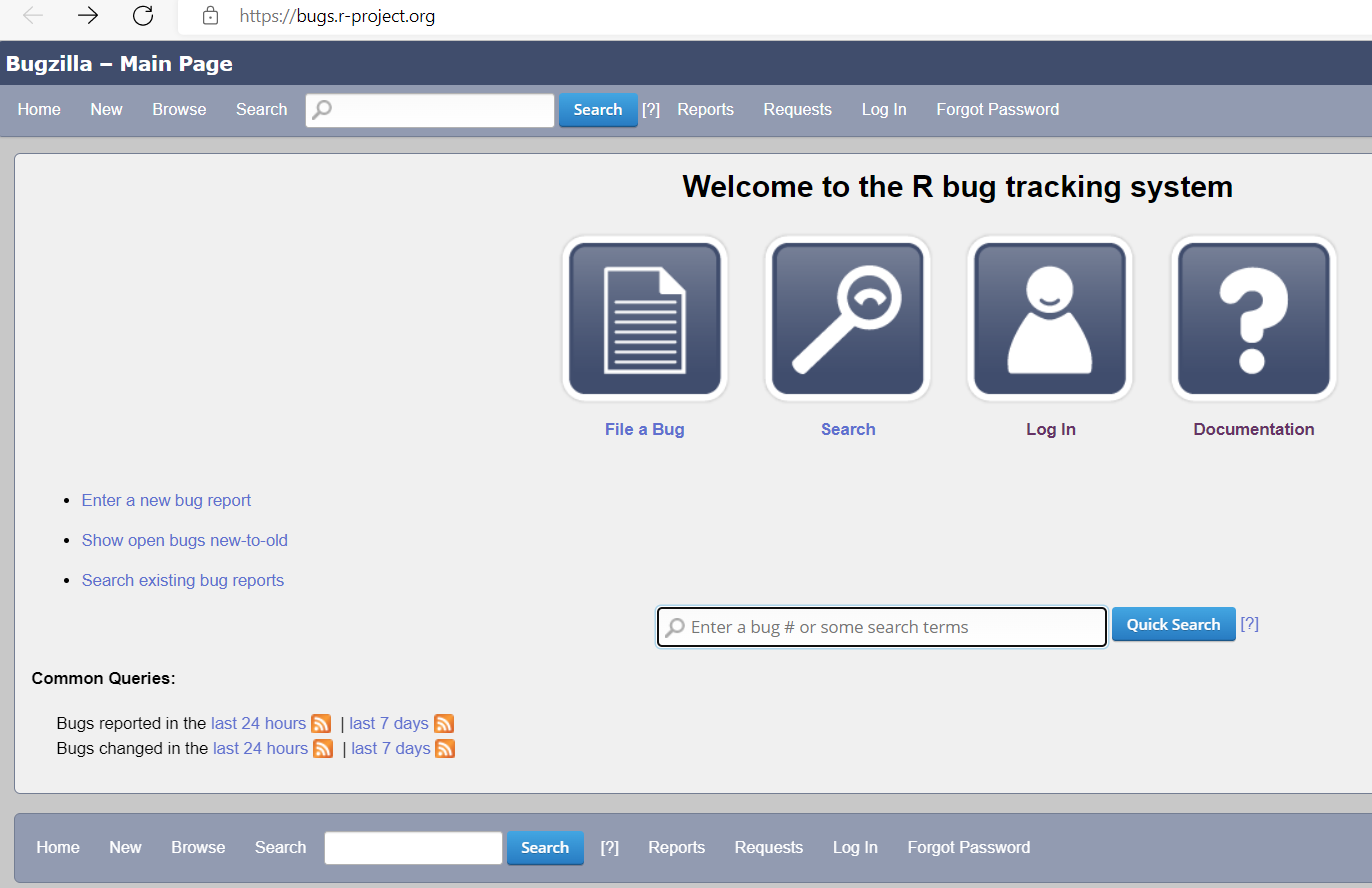
\includegraphics{img/bugzilla.png}
\caption{Screenshot of the existing home page of Bugzilla.}
\end{figure}

On the home page of Bugzilla, there are various buttons and links. There are four square buttons called as:

\begin{figure}
\centering
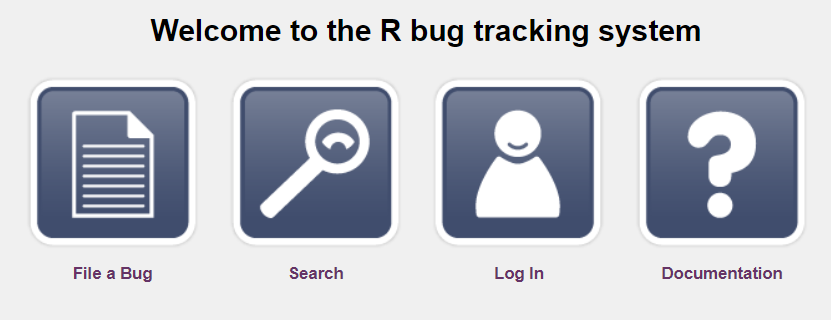
\includegraphics{img/squarebuttons.png}
\caption{Screenshot of the four square buttons on the home page of Bugzilla.}
\end{figure}

\begin{enumerate}
\def\labelenumi{\arabic{enumi}.}
\item
  \href{https://bugs.r-project.org/enter_bug.cgi}{File a bug}: You will have to log in to Bugzilla to file a bug using this button
\item
  \href{https://bugs.r-project.org/query.cgi}{Search}: When you click this button you will get a page with `Simple Search' and `Advanced Search' options. Either of the search options could be used depending on what you are looking for.
\item
  \href{https://bugs.r-project.org/?GoAheadAndLogIn=1}{Log In}: Provide the appropriate email address and password here to log in to Bugzilla.
\item
  \href{https://bugzilla.readthedocs.io/en/latest/using/index.html}{Documentation}: Provides a user guide for R\textquotesingle s Bugzilla.
\end{enumerate}

Several useful shortcuts are available from the landing page:

\begin{enumerate}
\def\labelenumi{\arabic{enumi}.}
\item
  \href{https://bugs.r-project.org/enter_bug.cgi}{Enter a new bug report}
\item
  \href{https://bugs.r-project.org/buglist.cgi?bug_file_loc_type=allwordssubstr&bug_status=NEW&bug_status=ASSIGNED&bug_status=CONFIRMED&bug_status=REOPENED&bug_status=UNCONFIRMED&bugidtype=include&chfieldto=Now&cmdtype=doit&emailassigned_to1=1&emailassigned_to2=1&emailcc2=1&emailreporter2=1&emailtype1=substring&emailtype2=substring&field0-0-0=noop&long_desc_type=substring&order=bugs.delta_ts\%20desc&query_format=advanced&short_desc_type=allwordssubstr&type0-0-0=noop}{Show open bugs new-to-old}
\item
  \href{https://bugs.r-project.org/query.cgi}{Search existing bug reports}
\end{enumerate}

A \href{https://bugs.r-project.org/page.cgi?id=quicksearch.html}{quick search} bar is available on the home page where you can enter a bug number to search or some search terms.

\begin{figure}
\centering

\includegraphics{img/quicksearch.png}
\caption{Screenshot of the quick search bar on the home page of Bugzilla.}
\end{figure}

There is also a section for Common Queries on the home page which includes links to bugs reported and changed in the last 24 hours and last 7 days.

\begin{figure}
\centering
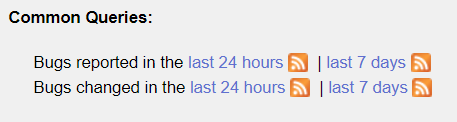
\includegraphics{img/commonquery.png}
\caption{Screenshot of the Common Queries section on the home page of Bugzilla.}
\end{figure}

\section{Searching for Bugs to Contribute to}\label{searching}

When presented with a long list of bugs, it can often be a bit demotivating when it's not clear where to start.
To help with this, you can use the \href{https://bugs.r-project.org/query.cgi?format=advanced}{\textbf{Advanced Search}}.

\begin{figure}
\centering
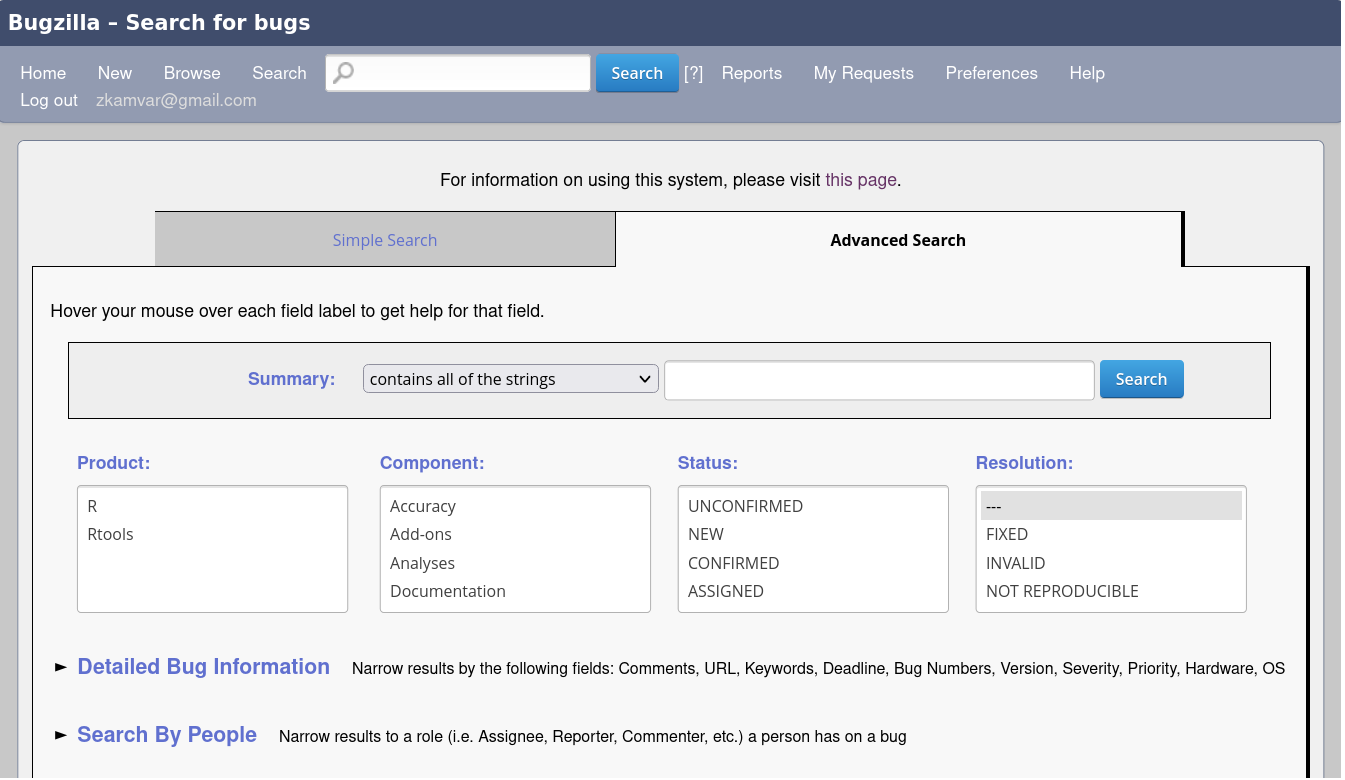
\includegraphics{img/bugzilla-adv-search-home.png}
\caption{Screenshot of Advanced Search page showing the following fields: Summary, Product, Component, Status, Resolution}
\end{figure}

This presents several fields that you can use to narrow down your search.
You can find out what a particular field is by clicking on the header, which will take you to that section in the \href{https://bugs.r-project.org/page.cgi?id=fields.html}{\textbf{Bug Fields Information Page}}.

The default fields are:

\begin{itemize}
\tightlist
\item
  \href{https://bugs.r-project.org/page.cgi?id=fields.html\#short_desc}{Summary}: a short description of the bug
\item
  \href{https://bugs.r-project.org/page.cgi?id=fields.html\#product}{Product}: either R or RTools.
\item
  \href{https://bugs.r-project.org/page.cgi?id=fields.html\#component}{Component}: A specific component of the R toolchain such as Graphics, Documentation, and Models
\item
  \href{https://bugs.r-project.org/page.cgi?id=fields.html\#bug_status}{Status}: The status of open or closed bugs. This will always default to showing open bugs (UNCONFIRMED, CONFIRMED, and IN\_PROGRESS)
\item
  \href{https://bugs.r-project.org/page.cgi?id=fields.html\#resolution}{Resolution}: The resolution for closed bugs.
\end{itemize}

You can select multiple items for each field as well.
Both \textbf{Product} and \textbf{Component} are what you navigate through when you go to \href{https://bugs.r-project.org/describecomponents.cgi}{\textbf{Browse Issues}}.

Below that are further filters that can help you find bugs you might want to work on:

\begin{description}
\tightlist
\item[Detailed Bug Information: Narrow results by the following fields]
Comments, URL, Keywords, Deadline, Bug Numbers, Version, Severity, Priority, Hardware, OS
Search By People

Narrow results to a role (i.e.~Assignee, Reporter, Commenter, etc.) a person has on a bug
Search By Change History

Narrow results to how fields have changed during a specific time period
Custom Search

Didn't find what you're looking for above? This area allows for ANDs, ORs, and other more complex searches.
\end{description}

These will be detailed in the subsections below

\subsection{Detailed Bug Information}\label{searching-dbi}

You can use this section to narrow down your search further to filter by things like OS type, R version, Keywords, and Priority.

It can be helpful, for example, to search for bugs labelled with \texttt{HELPWANTED}, which indicates bugs that may be suitable for anyone to work on regardless of expertise.

\begin{figure}
\centering
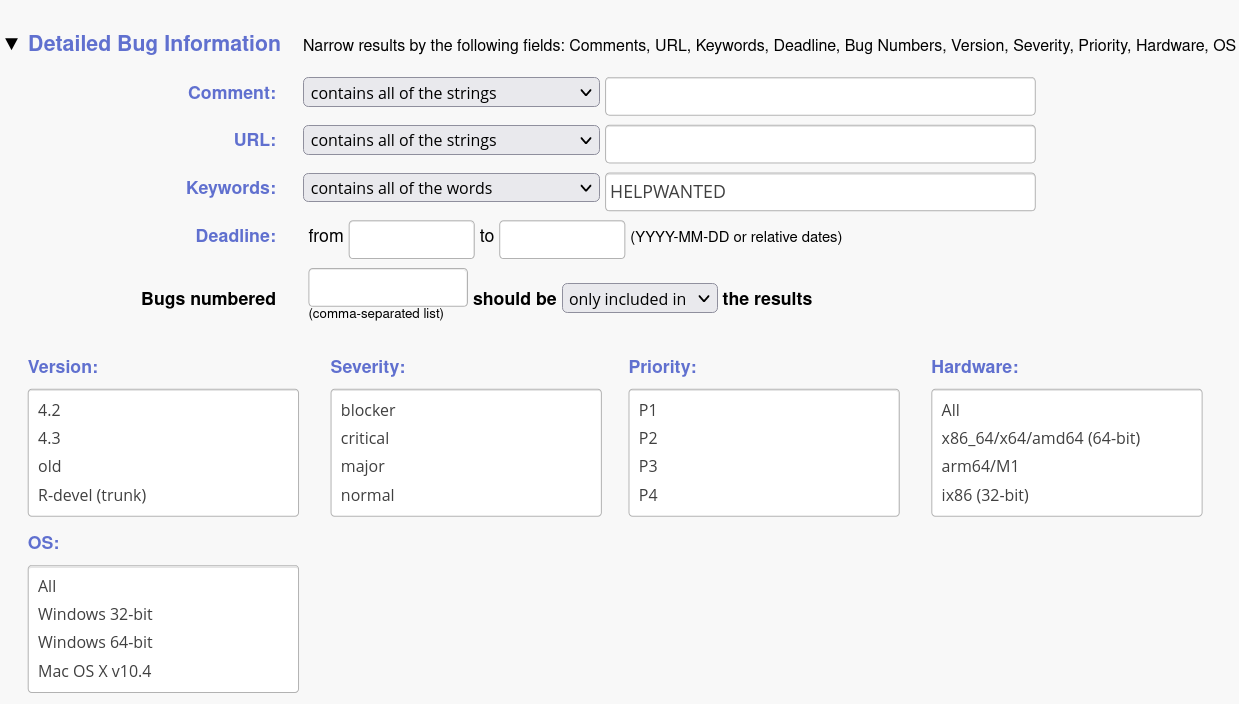
\includegraphics{img/bugzilla-adv-search-detailed-bug-info.png}
\caption{Screenshot of expanded Detailed Bug Information section showing the following fields: Comment, URL, Keywords (with HELPWANTED entered), Deadline, inclusion/exclusion of bug numbers, Version, Severity, Priority, Hardware, and OS}
\end{figure}

\subsection{Search By People}\label{searching-sbp}

You can use this to narrow down your search to only include results of a specific person or up to three people who have participated in any component of the bug's discusson.

\begin{figure}
\centering
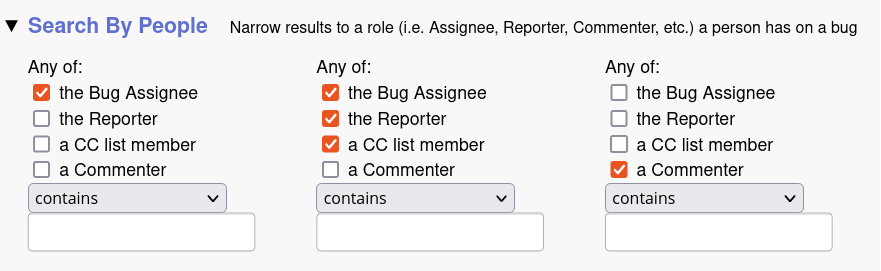
\includegraphics{img/bugzilla-adv-search-search-by-people.png}
\caption{Screenshot of expanded Search By People section showing three fields allowing you to enter a person's name who can be any of the bug assignee, the reporter, a CC list member, or a commenter}
\end{figure}

\subsection{Search By Change History}\label{searching-sbch}

Use this to search for bugs where any of the status fields has been changed (which, depending on the change, could indicate that someone from R-Core has given some attention to the bug).
This also provides a date range to narrow your search.

\begin{figure}
\centering
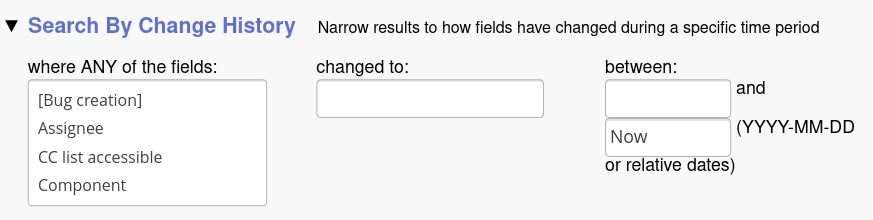
\includegraphics{img/bugzilla-adv-search-search-by-change-history.png}
\caption{Screenshot of expanded Search by Change History section showing three fields: where ANY of the fields (multi-select list), changed to, and between (dates in YYYY-MM-DD format)}
\end{figure}

\chapter{Reporting Bugs}\label{ReportingBugs}

\section{What is a bug in R?}\label{what-is-a-bug-in-r}

You may find a bug in R if:

\begin{enumerate}
\def\labelenumi{\arabic{enumi}.}
\tightlist
\item
  The R session terminates unexpectedly, or there is a segmentation fault, it might be a bug in R, unless you have written your own call to compiled code or an internal function (via \texttt{.C} or \texttt{.Internal}). The error may look like this:
\end{enumerate}

\begin{Shaded}
\begin{Highlighting}[]
\DocumentationTok{\#\#  *** caught segfault ***}
\DocumentationTok{\#\# address (nil), cause \textquotesingle{}memory not mapped\textquotesingle{}}
\end{Highlighting}
\end{Shaded}

\begin{enumerate}
\def\labelenumi{\arabic{enumi}.}
\setcounter{enumi}{1}
\tightlist
\item
  If the code does not do what the documentation says it should, then either the code or the documentation is wrong. Report either of which needs to be fixed.
\end{enumerate}

\textbf{Note}:
When you are in doubt that there is a bug: (which should be the case most of the time!)

\begin{enumerate}
\def\labelenumi{\arabic{enumi}.}
\item
  Make sure whether the bug appears in a clean session of R. Many times, there are variables/commands/functions stored in the workspace which might cause issues. Hence, check if the issue happens in a clean session. To do so, launch R from the command line with the \texttt{-\/-vanilla} option.
\item
  At times the code that is written is very complicated, has numerous package and file dependencies, has many function calls, etc.. In such scenarios it is quite common that the code throws an error and you are not able to solve it. You may tend to think that there is a bug that needs to be reported. Before doing so, try to produce a minimum working example of the code for the section where the error occurred. Add only those packages and files which are required by that section, and see if the error still appears. Using this approach shall solve most of the errors.
\item
  Install R-devel, which is the most recent version of R from \href{https://svn.r-project.org/R/trunk/}{svn} / \href{https://github.com/r-devel/r-svn}{git} or \href{https://cran.r-project.org/bin/windows/base/rdevel.html}{daily Windows build}, and see if your bug still exists in R-devel (it may have been fixed very recently).
\item
  \href{https://r.789695.n4.nabble.com/template/NamlServlet.jtp?macro=search_page&node=909078&query=isna&days=0}{Search on the R-devel mailing list for messages with keywords related to your possible bug}. If you find some related messages then read them to see if they clarify whether or not it is a bug. If you do not find any related messages, then please post a new message to R-devel. Your message should include (1) a brief description of the bug including current and expected behavior, (2) a minimal reproducible example.
\end{enumerate}

\section{What condition might not be a bug?}\label{what-condition-might-not-be-a-bug}

\begin{enumerate}
\def\labelenumi{\arabic{enumi}.}
\item
  In case the code is doing something unexpected, it may not necessarily be a bug. Carefully review the documentation of the function being called, and check whether the behaviour being exhibited on calling this function is the same as it was designed to do.
\item
  Issues with \href{https://cran.r-project.org/doc/FAQ/R-FAQ.html\#Why-doesn_0027t-R-think-these-numbers-are-equal_003f}{\emph{seemingly} identical numbers} not being equal (especially floating point numbers) are usually not bugs.
\item
  If R is running slower than expected, then this also may not be a bug. Ask someone else to review your code in such a case.
\item
  If some function is working, but it is not defined in the best generalised way, then consult someone to look over the code. This may perhaps not be a bug; instead, it might be an alternative way of writing the function.
\end{enumerate}

\section{Checking if a bug is already reported}\label{checking-if-a-bug-is-already-reported}

The first step before filing a bug report is to see whether the problem has already been reported. Checking if the bug is reported will:

\begin{enumerate}
\def\labelenumi{\arabic{enumi}.}
\item
  Save time for you and the developers.
\item
  Help you see if the bug is already fixed for the next release.
\item
  Lead you to learn what needs to be done to fix it.
\item
  Determine if any additional information is needed.
\end{enumerate}

The sections that follow discuss where to check whether a bug is already reported.

\section{What are some places where you may find a bug?}\label{what-are-some-places-where-you-may-find-a-bug}

You may find a bug in:

\begin{enumerate}
\def\labelenumi{\arabic{enumi}.}
\item
  In the \hyperref[RCorePkgBug]{R-Core supported packages, their documentations, and/ or in the R language implementation}.
\item
  In \hyperref[nonRCorePkgBug]{packages and/or their documentations which are not supported by the R-Core}.
\end{enumerate}

\section{How to report a bug?}\label{ReportBug}

Once you confirm a bug exists, you need to submit a bug report so that it gets fixed.

\subsection{Bug in the R-Core supported packages, their documentations, and/ or in the R language}\label{RCorePkgBug}

\begin{enumerate}
\def\labelenumi{\arabic{enumi}.}
\item
  Packages that are supported by the R-Core are labelled with \texttt{Maintainer:\ R\ Core\ Team\ \textless{}R-core@r-project.org\textgreater{}}. One simple way to get the information from R is by running the \texttt{maintainer("package\_name")} command.
\item
  The bug report for R-Core supported packages, their documentations, and/ or a bug report for the R language itself can be submitted either to R-devel, \href{https://www.r-project.org/posting-guide.html\#which_list}{see posting guide}, or to \href{https://bugs.r-project.org/bugzilla/}{Bugzilla}. In the future, we hope to have an option to report an issue to the \href{https://github.com/r-devel/r-svn/issues}{GitHub Mirror of the R svn server}.
\item
  In order to report bugs, as well as fixes, using \hyperref[Bugzilla]{Bugzilla}, please ensure that you have a \hyperref[bugzilla-account]{Bugzilla account}
\item
  Please ensure whether the bug is already fixed (in the upcoming changes in R) or reported (search for it from those already reported on Bugzilla, either on \href{https://bugs.r-project.org/bugzilla/query.cgi}{search existing bug reports}, using the \href{https://bugs.r-project.org/bugzilla/query.cgi?format=advanced}{advanced search} option here, or \href{https://bugs.r-project.org/bugzilla/buglist.cgi?bug_file_loc_type=allwordssubstr&bug_status=NEW&bug_status=ASSIGNED&bug_status=CONFIRMED&bug_status=REOPENED&bug_status=UNCONFIRMED&bugidtype=include&chfieldto=Now&cmdtype=doit&emailassigned_to1=1&emailassigned_to2=1&emailcc2=1&emailreporter2=1&emailtype1=substring&emailtype2=substring&field0-0-0=noop&long_desc_type=substring&order=bugs.delta_ts\%20desc&query_format=advanced&short_desc_type=allwordssubstr&type0-0-0=noop}{show open bugs new-to-old}).
\end{enumerate}

\subsection{Bug in the non R-Core supported packages and/or their documentations}\label{nonRCorePkgBug}

For packages that are not maintained by the R-Core, the bug reports can be submitted at, perhaps, an issues tracker url on GitHub/GitLab/R-Forge. To find if such an issues tracker is available, you can look at the package \texttt{DESCRIPTION} file first (e.g.~using \texttt{packageDescription("package\_name")}) to check if a url is provided in the \texttt{BugReports} field. If that is not available, then the package maintainer can be contacted (using \texttt{maintainer("package\_name")}). In R running the function \texttt{bug.report(package\ =\ "package\_name")} shall direct you to either the GitHub issue tracker of the package, or to the bug tracking web page, or towards composing an e-mail to the package maintainer. This function \texttt{bug.report} is disabled in RStudio, by default. However, if you use \texttt{utils::bug.report(package\ =\ "package\_name")} then it works on RStudio as well. Please ensure that the bug is not already reported or fixed before reporting it in any of the ways suggested above.

\section{Good practices in reporting bugs / Expectations of a good bug report}\label{good-practices-in-reporting-bugs-expectations-of-a-good-bug-report}

If you follow the practices given below, you will come up with a good bug report which might make it easier for the maintainer(s) to fix the bug.

\begin{enumerate}
\def\labelenumi{\arabic{enumi}.}
\item
  Include a minimal reproducible example of the bug in your report. The maintainer should be able to quickly reproduce the bug using the minimal example that you provide. Here is a \href{https://stackoverflow.com/questions/5963269/how-to-make-a-great-r-reproducible-example}{community wiki post} on how to make a minimal reproducible example.
\item
  Mention the software architecture on which the bug occurred.
\item
  Use inbuilt data sets as far as possible.
\end{enumerate}

In addition to the above, here are the \href{https://bugs.r-project.org/bugzilla/page.cgi?id=bug-writing.html}{bug writing guidelines} on Bugzilla. The \href{https://www.r-project.org/bugs.html\#writing-a-good-bug-report}{bug reporting} documentation in R also discusses practices to write a good bug report.

Once you have successfully reported a bug, you will likely receive an update each time an action is taken on the bug. On Bugzilla, the report may be given one of the following status: New, Assigned, Confirmed, Reopened, Unconfirmed.

\section{Disagreement with a resolution on the bug tracker}\label{disagreement-with-a-resolution-on-the-bug-tracker}

As humans, there might be differences of opinions from time to time. What needs to be considered here is to be respectful of the fact that care, thought, and volunteer time has gone into the resolution of the issue or bug.

If you take some time, then on reflection, the resolution steps may seem more reasonable than you initially thought. If you still feel that the resolution is incorrect, then raise a thoughtful question to the person who resolved it. If the issue was not carefully thought about in the first place then it is less likely to win any conversion of thought.

As a reminder, issues closed by a core developer on Bugzilla have already been carefully considered. Please do not reopen a closed issue. Although one can comment on a closed issue, if necessary. Every comment on an issue generates an email to every R-core member (unless they have the notifications disabled). So it would be best to be considerate while commenting on issues, especially in case of closed issues or when you are commenting in pure agreement without adding anything beyond that to a discussion (the +1 type posts which are perfectly acceptable in other contexts).

\section{Examples of Bug reports submitted on Bugzilla or R-devel mailing list}\label{examples-of-bug-reports-submitted-on-bugzilla-or-r-devel-mailing-list}

If you like to see how bugs are reported on Bugzilla, here are some examples:

\begin{enumerate}
\def\labelenumi{\arabic{enumi}.}
\item
  \href{https://bugs.r-project.org/bugzilla/show_bug.cgi?id=17767}{Bug 17767 - Warning about incomplete argument within nlme}: A bug report with a reproducible example, a patch, and a review.
\item
  \href{https://stat.ethz.ch/pipermail/r-devel/2019-May/077855.html}{Possible bug when finding shared libraries during staged installation}: A bug report submitted by Kara Woo which was promptly fixed via the R-devel mailing list. (More information about the R-devel mailing list can be found \href{https://stat.ethz.ch/mailman/listinfo/r-devel}{here}).
\item
  \href{https://stat.ethz.ch/pipermail/r-devel/2019-February/077393.html}{Bug: time complexity of substring is quadratic as string size and number of substrings increases}: A substring reported by Toby Dylan Hocking and fixed by Tomas Kalibera, Feb 2019 via the R-devel mailing list.
\item
  \href{https://stat.ethz.ch/pipermail/r-devel/2019-February/077315.html}{patch for gregexpr(perl=TRUE)}: A gregexpr bug report and patch submitted by Toby Dylan Hocking and merged by Tomas Kalibera, Feb 2019 via the R-devel mailing list.
\end{enumerate}

\section{See also}\label{see-also-1}

\begin{enumerate}
\def\labelenumi{\arabic{enumi}.}
\item
  \href{https://www.r-project.org/bugs.html}{Reporting a bug}
\item
  \href{https://mac.r-project.org/man/R-FAQ.html\#R-Bugs}{R FAQ on bugs}
\item
  \href{https://bugs.r-project.org/bugzilla/page.cgi?id=bug-writing.html}{Bugzilla guidelines of reporting a bug}
\end{enumerate}

\chapter{Reviewing Bugs}\label{ReviewBugs}

\section{How you can help to review bug reports?}\label{how-you-can-help-to-review-bug-reports}

After understanding where bugs are reported in R (Bugzilla) or in other projects (GitHub/GitLab/R-Forge), a great way to contribute is reviewing bug reports.

Around the clock, new bug reports are being submitted on Bugzilla or the bug trackers (for instance, GitHub issues) of R packages and existing bug reports are being updated. Every bug report needs to be reviewed to make sure various things are in proper order. You can help with this process of reviewing bugs.

\subsection{Preparing to review bug reports}\label{preparing-to-review-bug-reports}

If you want to review bug reports on Bugzilla, you are required to have a \hyperref[bugzilla-account]{Bugzilla account}. More details on how you can review a bug report are available on this post on the R Blog: \href{https://blog.r-project.org/2019/10/09/r-can-use-your-help-reviewing-bug-reports/index.html}{R Can Use Your Help: Reviewing Bug Reports}

\section{Classifying bug reports}\label{classifying-bug-reports}

A good bug report is the one which:

\begin{enumerate}
\def\labelenumi{\arabic{enumi}.}
\item
  Explains clearly how to reproduce the bug.
\item
  Includes the version of R, the machine architecture, and the operating system platform on which the bug occurred.
\end{enumerate}

Relevant details should be a part of a good bug report. You can help with the following tasks once you have some R programming experience:

\begin{enumerate}
\def\labelenumi{\arabic{enumi}.}
\item
  Reproducing the bug: If you see a bug report which does not clearly explain how to reproduce it, you can try reproducing the bug and eventually make things easier for the core developer(s) and/or package maintainer(s).
\item
  Checking different binary builds: Check whether the bug occurs on a different binary build of R. It is helpful to know whether the bug is affecting: \texttt{r-patched}, \texttt{r-devel}, or \texttt{r-release} binary builds of R.
\item
  Writing a unit test: If the bug report lacks a unit test that should be a part of R's test suite, then you can help with providing it.
\end{enumerate}

These helpful tasks allow the Core developers and/ or maintainers to classify a bug report properly, so that the bug can be handled in a timely fashion.

\section{How to find a bug report or an issue to review?}\label{how-to-find-a-bug-report-or-an-issue-to-review}

\begin{enumerate}
\def\labelenumi{\arabic{enumi}.}
\item
  You may search old bug reports or issues that could be closed. Old bug reports may no longer be valid or may include a patch that is ready to be committed, but no one has had the time to review and commit.
\item
  You might also want to search for issues in topics in which you have a working knowledge. When on Bugzilla you can use the advanced search to find specific topics. Bug reports are by default public on Bugzilla (unless the defaults are changed to avoid security vulnerability).
\end{enumerate}

\section{Example of a bug review submitted on Bugzilla}\label{example-of-a-bug-review-submitted-on-bugzilla}

If you would like to see how bugs are reviewed on Bugzilla, the \href{https://bugs.r-project.org/bugzilla/show_bug.cgi?id=16542}{Bug 16542 - nlme:::summary.lmList with unequal outputs per group} is an example where an old bug report is being reviewed. It is tested to see if it was still an issue and a few ways are proposed to resolve the issue.

\textbf{Note}:

There is a \texttt{\#bug-reporting} channel on the \href{https://r-contributors.slack.com/}{R Contributors slack} where you can share your bug report(s) for review/feedback before submitting to Bugzilla. This can help with checking that it really is a bug, that you have included the important information and excluded redundant information.

\section{See also}\label{see-also-2}

\begin{enumerate}
\def\labelenumi{\arabic{enumi}.}
\tightlist
\item
  \href{https://blog.r-project.org/2019/10/09/r-can-use-your-help-reviewing-bug-reports/index.html}{Reviewing bug reports: Blog}
\end{enumerate}

\chapter{Finding the Source}\label{FindSource}

This chapter discusses how you can have an overview of the R codebase. For instance, where to find the implementation of a base function written in R and where to find a primitive implementation written in C. You may want to find the source code of a function just out of curiosity or maybe to gain more insight into what a particular function is actually doing. Whatever be the case, reading the source code will help you to learn a lot about any function.

\section{Finding R source code}\label{finding-r-source-code}

\begin{enumerate}
\def\labelenumi{\arabic{enumi}.}
\tightlist
\item
  Find the R function with the code of interest. You will always be able to print the top-level function (or use \texttt{View(function\_name)} in RStudio). Looking at the code for the body of this function will reveal what you need to do next:
\end{enumerate}

\begin{itemize}
\item
  Can already see code of interest: stop here or skip to step 3 to find the corresponding file in the R sources.
\item
  Code of interest is in nested R function: go to step 2.
\item
  Top-level function is an S3 generic, identified by a call to \texttt{UseMethod()}. Use \texttt{methods(function\_name)} to see available methods, then go to step 2.
\item
  Code of interest is in compiled code, identified by a call to \texttt{.C()}, \texttt{.Call()}, \texttt{.Fortran()}, and \texttt{.External()}, or \texttt{.Internal()} and \texttt{.Primitive()}: go to section on compiled code.
\end{itemize}

\begin{enumerate}
\def\labelenumi{\arabic{enumi}.}
\setcounter{enumi}{1}
\item
  Nested functions or S3 methods may not be exported by the package they are in. If this is the case, the simplest way to view the code is to use \texttt{getAnywhere()} or \texttt{getS3method()}. Now you can keep looking at nested R functions till you find the code of interest or hit a call to compiled code.
\item
  Find an R function in the R sources. Two options here:
\end{enumerate}

\begin{itemize}
\tightlist
\item
  Search on the internet: For R Core packages, search on the GitHub mirror (\url{https://github.com/r-devel/r-svn}); for recommended packages, use the CRAN mirror (\url{https://github.com/cran}) - this will link to the source on GitHub if available, e.g.~\url{https://github.com/cran/survival}. Note that GitHub search ignores wildcard characters
\end{itemize}

\begin{verbatim}
 . , : ; / \ ` ' " = * ! ? # $ & + ^ | ~ < > ( ) { } [ ]
\end{verbatim}

but this does not include \texttt{-} so you can search for a function or S3 method as follows:

\begin{verbatim}
"body <- function" extension:R
"quantile.ecdf <- function" extension:R
\end{verbatim}

\begin{itemize}
\tightlist
\item
  Search in the R sources using grep: The \hyperref[GetStart]{Getting Started} chapter discusses how to download the R sources directly or from the svn repository. Now if the sources are in \texttt{\textasciitilde{}/R-devel}, you can search as follows:
\end{itemize}

\begin{verbatim}
grep -R "body <- function" ~/R-devel/src
grep -R "quantile <- function" ~/R-devel/src/library
\end{verbatim}

Note: The above procedure does not cover S4, R6 or RC generics or methods. Refer \href{https://github.com/jennybc/access-r-source}{accessing R source} for further details.

\section{Finding C source code}\label{finding-c-source-code}

\begin{enumerate}
\def\labelenumi{\arabic{enumi}.}
\tightlist
\item
  If \texttt{.Internal()} or \texttt{.Primitive()}, find entry point in \texttt{names.c} as described in the Jenny Bryan's post of \href{https://github.com/jennybc/access-r-source}{accessing R source}. For all other calls to compiled code, you can find the entry point from within R. For instance, the body of complete.cases() is
\end{enumerate}

\begin{verbatim}
.External(C_compcases, ...)
\end{verbatim}

\texttt{C\_compcases} inherits from class ``NativeSymbolInfo'' and we can extract the name of the entry point via

\begin{verbatim}
stats:::C_compcases$name
\end{verbatim}

We know that it is in the stats package as we see that when we print complete.cases or look at the help file. This shows us that the entry point is simply ``compcases'' and in fact that is the general convention in R code, that you simply remove the \texttt{C\_} prefix (sometimes \texttt{.F\_} for Fortran code) in the name of the object passed to the first argument of the call.

\begin{enumerate}
\def\labelenumi{\arabic{enumi}.}
\setcounter{enumi}{1}
\tightlist
\item
  Once you have the entry point, search as for R code. In the case of searching on GitHub, restrict the search to files with the relevant extension
\end{enumerate}

\begin{verbatim}
compcases path:*.c
lowesw path:*.f
\end{verbatim}

similarly for grep

\begin{verbatim}
grep -R --include=*.c "compcases" ~/R-devel/src/library/
\end{verbatim}

Note:

\begin{enumerate}
\def\labelenumi{\arabic{enumi}.}
\item
  Many editors (like RStudio, ESS) support \href{https://en.wikipedia.org/wiki/Ctags}{ctags} for code browsing, making it easy to jump to definitions of functions. \texttt{R\ CMD\ rtags} can generate ctags for any R code (Credit: Deepayan Sarkar).
\item
  A more sophisticated system is called GNU GLOBAL, which also supports
  finding all references (calls) to a function.
\item
  GitHub has a code navigation feature via the library tree-sitter. Unfortunately, it does not have R support yet. An \href{https://github.com/r-lib/tree-sitter-r}{R driver for tree-sitter} made by Jim Hester is available.
\end{enumerate}

\section{See also}\label{see-also-3}

\href{https://blog.r-hub.io/2019/05/14/read-the-source/}{Read the R source} blogpost.

\chapter{Lifecycle of a Patch}\label{FixBug}

\section{Introduction}\label{introduction-1}

R uses a workflow based on patches. A patch is the set of differences (additions and deletions) between two versions of code. So you can create a patch defining a bug fix or a proposed update to the R codebase and submit it through your official Bugzilla account to the core developer(s). Be clear in your communication as it is the key to contributing to any project, especially an open source project like R.

\section{When do you submit a patch?}\label{when-do-you-submit-a-patch}

There might be a situation where you come across a bug in R, which you may have an idea of how to fix. This can turn out to be an opportunity for you to submit a patch. By submitting a patch or a bug fix, you are helping to reduce the workload on the R developers in addition to yourself being a contributor to R!

When you submit a patch, you are helping the developer(s) and maintainer(s) so that they do not have to write the entire code from scratch. Instead, they can test and tweak your patch, if necessary.

\section{What tools are required to submit a patch?}\label{what-tools-are-required-to-submit-a-patch}

To submit a patch, you need:

\begin{enumerate}
\def\labelenumi{\arabic{enumi}.}
\item
  \href{http://subversion.apache.org/}{SVN} installed on your machine.
\item
  The latest developer version of R.
\end{enumerate}

You can retrieve the latest source code of R via:

\begin{Shaded}
\begin{Highlighting}[]
\BuiltInTok{export} \VariableTok{TOP\_SRCDIR}\OperatorTok{=}\StringTok{"}\VariableTok{$HOME}\StringTok{/Downloads/R"}
\FunctionTok{svn}\NormalTok{ checkout https://svn.r{-}project.org/R/trunk/ }\StringTok{"}\VariableTok{$TOP\_SRCDIR}\StringTok{"}
\end{Highlighting}
\end{Shaded}

Depending on the operative system you might need to do some steps before that.
The different steps required can be found in previous chapters of the book, for \hyperref[windowsSource]{Windows}, \hyperref[macos]{macOS} and \hyperref[linux]{Linux}.

\section{How to prepare a patch?}\label{how-to-prepare-a-patch}

If you have the source code in \texttt{\$TOP\_SRCDIR} you can edit the files, for example a documentation file such as \texttt{"\$TOP\_SRCDIR"/src/library/stats/man/Multinom.Rd}, to make your desired changes to that or more files.

Then you should check that R still works as expected via:

\begin{Shaded}
\begin{Highlighting}[]
\BuiltInTok{cd} \StringTok{"}\VariableTok{$TOP\_SRCDIR}\StringTok{"}
\FunctionTok{make}\NormalTok{ check{-}devel}
\end{Highlighting}
\end{Shaded}

If there is no test for your proposed change you can add a new regression test, following \hyperref[TestR]{the guidelines}.

Then you should bring changes from the repository into the working copy, in case any other change has been introduced, and create a patch.diff file with just the changes you want to propose to the R core:

\begin{Shaded}
\begin{Highlighting}[]
\FunctionTok{svn}\NormalTok{ update}
\FunctionTok{svn}\NormalTok{ diff }\OperatorTok{\textgreater{}}\NormalTok{ patch.diff}
\end{Highlighting}
\end{Shaded}

Most often, changes are made to existing files, but if you happen to be adding a new file in your change, you'll need to run \texttt{svn\ add\ path/to/file1\ ...} before running \texttt{svn\ diff} to mark those files for inclusion.

This \texttt{patch.diff} file is the one that can be proposed to the R core via \hyperref[SubmitPatches]{Bugzilla}. You can also \hyperref[PatchesReview]{ask for reviews} to the patch before proposing it to the R core via the \href{https://stat.ethz.ch/mailman/listinfo/r-devel}{r-devel mailing list} or the slack channel of the R-contributors space.

\subsection{Using a git mirror}\label{using-a-git-mirror}

Besides checking in your computer, you can use the Github mirror \href{https://github.com/r-devel/r-svn}{r-devel/r-svn} of the source code to check this patch with different configurations and OS.

You should first find the file to edit, via the github interface for example:

\begin{figure}
\centering
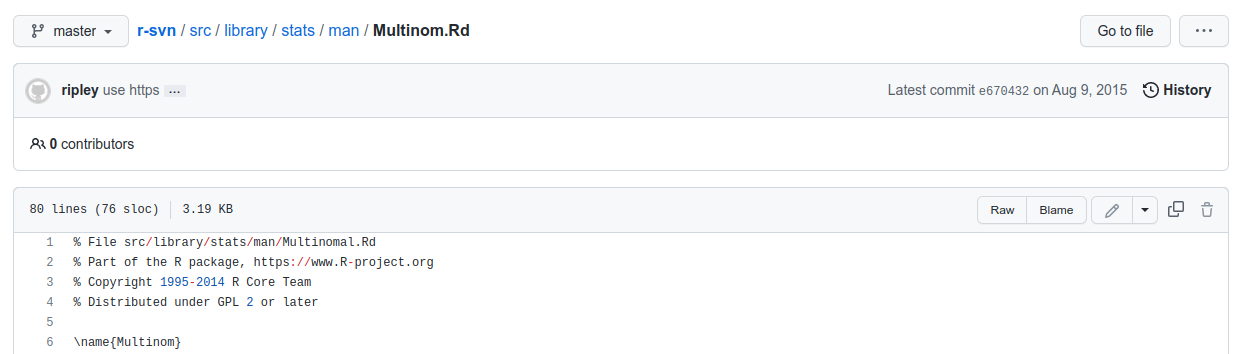
\includegraphics{img/rsvn_file_to_edit.png}
\caption{Screenshot of the heading of the src/library/stats/man/Mulinom.Rd}
\end{figure}

Then you can edit it, directly in the interface or using the github interface:

\begin{figure}
\centering
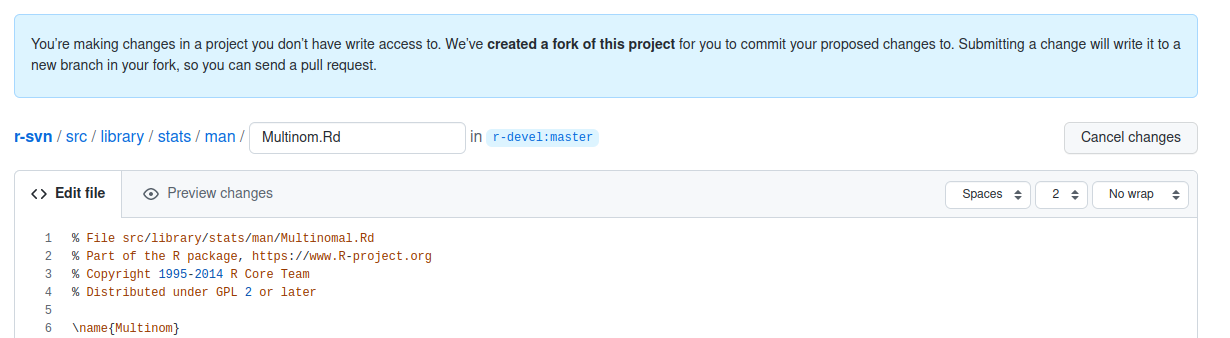
\includegraphics{img/rsvn_edit_file.png}
\caption{Screenshot of the file src/library/stats/man/Mulinom.Rd being edited via the Github interface}
\end{figure}

Create a commit with a message describing the changes

\begin{figure}
\centering
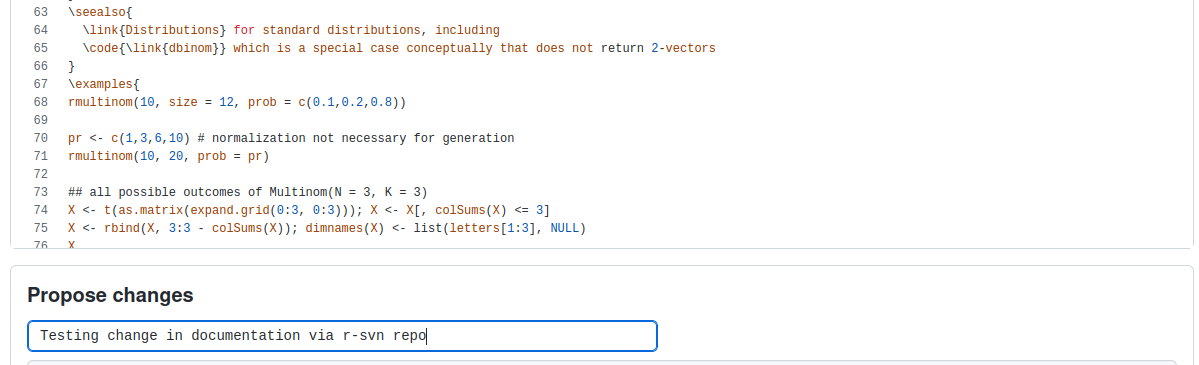
\includegraphics{img/rsvn_commit_message.png}
\caption{Screenshot of the commit message}
\end{figure}

And create a pull request from the branch created to check the changes.

\begin{figure}
\centering
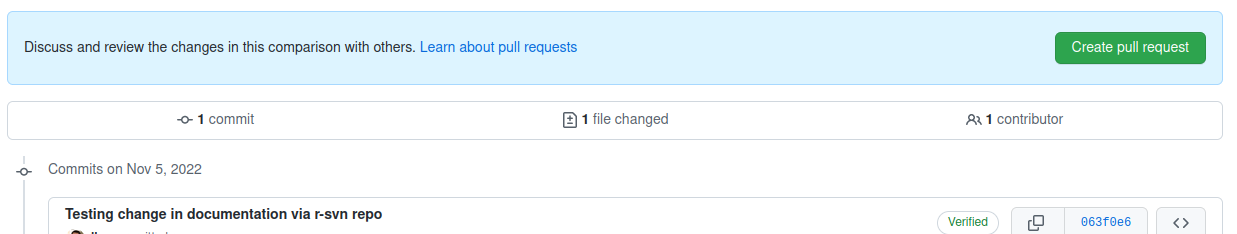
\includegraphics{img/rsvn_commit_pre_PR.png}
\caption{Screenshot of the message when opening a pull requests from the branch}
\end{figure}

Add a message and description of the svn for other users and the R core to know what is the purpose of this modification:

\begin{figure}
\centering
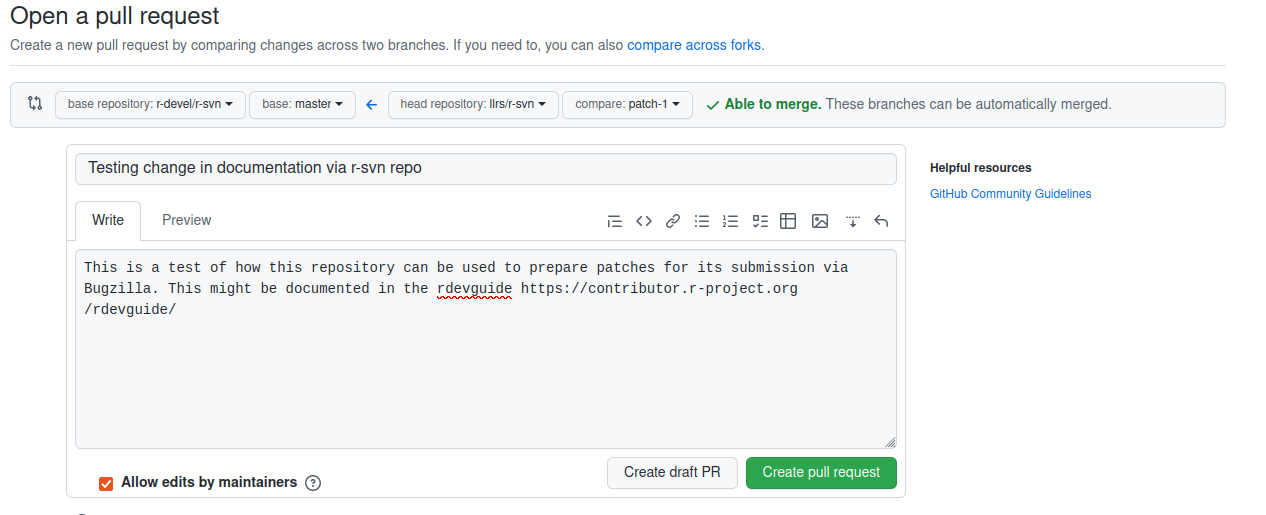
\includegraphics{img/rsvn_PR_message.png}
\caption{Screenshot of the message and content while opening a pull requests for the r-svn repository}
\end{figure}

\begin{figure}
\centering
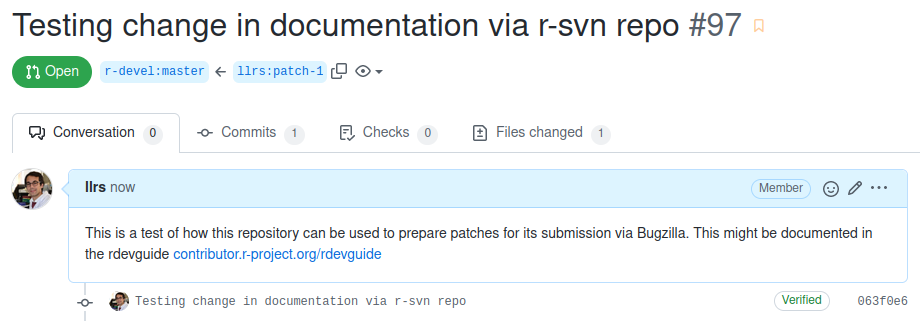
\includegraphics{img/rsvn_PR_created.png}
\caption{Screenshot of the pull requests opened}
\end{figure}

Once the PR is submitted, some automatic checks will be triggered (they might need to be approved by some other users as per Github rules):

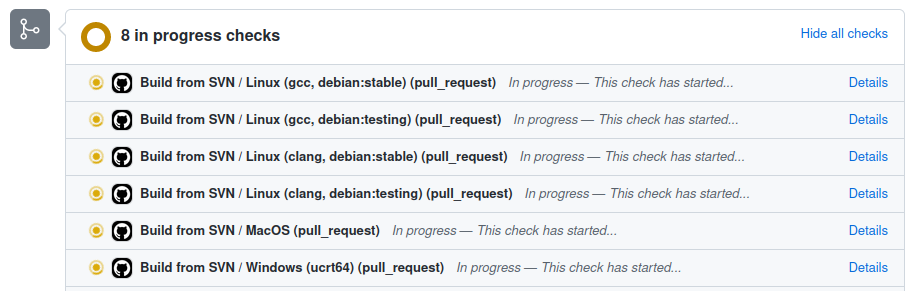
\includegraphics{img/rsvn_PR_automatic_checks.png}
When the checks end you will need to explore the results and asses if the results indicate a problem or not.

\begin{figure}
\centering
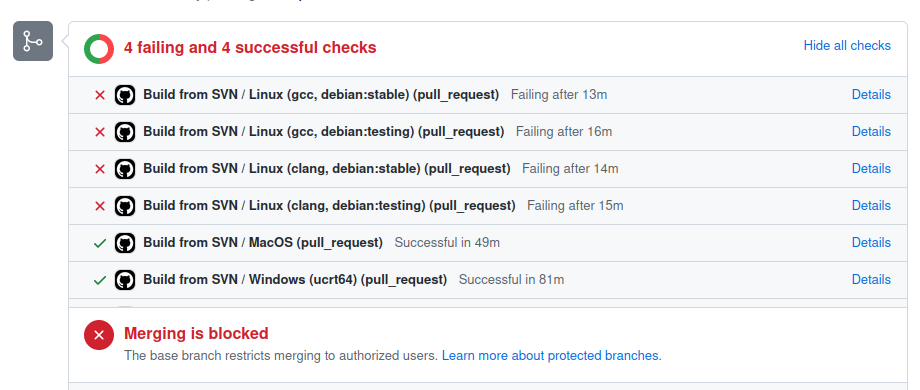
\includegraphics{img/rsvn_checks_results.png}
\caption{Screenshot of the results of the Github checks in the r-svn mirror}
\end{figure}

Once you are happy with the changes and the checks report that everything is okay you can retrieve the patch via:

\texttt{https://patch-diff.githubusercontent.com/raw/r-devel/r-svn/pull/\textless{}pull\_request\_number\textgreater{}.diff}

With that file you can \hyperref[SubmitPatches]{submit your patch}, remember to check if it meets the \hyperref[GoodPatches]{recommendations for good patches}.

If you want to use \texttt{git} from the terminal to create the pull request (PR) to test the changes, you can use this \href{https://about.gitlab.com/images/press/git-cheat-sheet.pdf}{summary of the available git commands}.

\section{Making good patches}\label{GoodPatches}

When creating a patch for submission, there are several things that you can do to help ensure that your patch is accepted:

\begin{enumerate}
\def\labelenumi{\arabic{enumi}.}
\item
  Make sure to follow \href{https://cran.r-project.org/doc/manuals/r-release/R-ints.html\#R-coding-standards}{R's coding standards} (R is a GNU project and there are GNU coding standards). The coding style of the patch you submit should largely match with the codebase it is being applied to. If your patch has one or two minor discrepancies, then those may be fixed by the core developer who will eventually test your patch. However, if there are systematic deviations from the style guides your patch will be put on hold until you fix the formatting issues. There is no comprehensive official R style manual, however some nearly universal standards are summarised in \href{https://cran.r-project.org/web/packages/rockchalk/vignettes/Rstyle.pdf}{this article}.
\item
  Be aware of backwards-compatibility considerations. While the core developer who eventually handles your patch will make the final call on whether something is acceptable, thinking about backwards-compatibility early will help prevent having your patch rejected on these grounds. Put yourself in the shoes of someone whose code will be broken by the change(s) introduced by the patch. It is quite likely that any change made will break someone's code, so you need to have a good reason to make a change as you will be forcing someone to update their code. This obviously does not apply to new functions or new arguments. New arguments should be optional and have default values which maintain the existing behaviour. If in doubt, \hyperref[WhereToGetHelp]{discuss} the issue with experienced developers.
\item
  Make sure you have proper tests to verify that your patch works as expected. Patches may not be accepted without the proper tests.
\item
  Make sure the entire test suite runs without failure because of your changes. It is not sufficient to only run whichever test seems impacted by your changes, because there might be interactions unknown to you between your changes and some other part of the interpreter.
\item
  Proper documentation additions/changes should be included.
\item
  Each bugfix should ideally be addressed by a single patch. In particular, do not fix more than one issue in the same patch (except, if one code change fixes all of them) and do not do cosmetic changes to unrelated code in the same patch as some bugfix.
\end{enumerate}

\section{Submitting your patch for review}\label{SubmitPatches}

\begin{enumerate}
\def\labelenumi{\arabic{enumi}.}
\item
  Patch in response to a pre-existing issue or bug report: In this case, you should attach the patch to the existing issue or bug report on Bugzilla with a brief comment.
\item
  Patch in response to an unreported issue or bug report: Assuming you already performed a search on Bugzilla for a pre-existing issue or bug and did not find the issue or bug reported, you need to create a new bug report and include your patch with it. Please fill in as much relevant detail as possible to prevent reviewers from having to delay reviewing your patch because of lack of information. Include (mostly as the first sentence), a to-the-point explanation of what the purpose of the patch is. This sentence should not be in the descriptive form, rather an imperative form will be more suitable here. If this is not enough detail for a patch, a new paragraphs(s) can be added to explain in proper depth what has happened. The details should be good enough that a core developer reading it understands the justification for the change.
\end{enumerate}

\section{Getting your patch reviewed}\label{PatchesReview}

To begin with, please be patient. There are many more people submitting patches than there are people capable of reviewing your patches. Getting your patch reviewed requires a reviewer to have the spare time and motivation to look at your patch. We cannot force anyone to review patches and no one is employed to look at patches.

There is a \texttt{\#patches-for-review} channel on the \href{https://r-contributors.slack.com/}{R Contributors slack} where you can share your patch(es) for review/feedback before submitting to R-Core/Bugzilla. This can help with checking that you have included the important information and excluded redundant information.

If your patch has not received any notice from reviewers (i.e., no comment made) after one month, comment/message on the \texttt{\#patches-for-review} channel to remind the members that the patch needs a review.

When someone does manage to find the time to look at your patch they will most likely make comments about how it can be improved. It is then expected that you update your patch to address these comments, and the review process will thus iterate until a satisfactory solution has emerged.

\subsection{How to review a patch?}\label{how-to-review-a-patch}

One of the bottlenecks in the R development process is the lack of code reviews. If you browse Bugzilla, you will see that numerous issues have a fix, but cannot be merged into the main source code repository, because no one has reviewed the proposed solution. Reviewing a patch can be just as informative as providing a patch and it will allow you to give constructive comments on another developer's work. This guide provides a checklist for submitting a patch review. It is a common misconception that in order to be useful, a patch review has to be perfect. This is not the case at all. It is helpful to just test the patch and/or play around with the code and leave comments in the patch or on Bugzilla.

If a bug report or an issue has a patch attached that has not been reviewed, you can help by making sure that the patch:

\begin{itemize}
\item
  follows the style guides;
\item
  is a good solution to the problem it is trying to solve;
\item
  includes proper tests; and
\item
  includes proper documentation changes.
\end{itemize}

Also refer to \hyperref[GoodPatches]{Making good patches} for more ideas. Doing all of this allows the core developer(s) and/ or maintainer(s) to more quickly look for subtle issues that only people with extensive experience working on R's codebase will notice.

\section{Leaving a patch review on Bugzilla}\label{leaving-a-patch-review-on-bugzilla}

When you review a patch, you should provide additional details and context of your review process and leave comments. For example:

\begin{enumerate}
\def\labelenumi{\arabic{enumi}.}
\item
  If you tested the patch, report the result and the system and version tested on, such as `Windows 10', `Ubuntu 16.4', or `Mac High Sierra'.
\item
  If you request changes, try to suggest how or attach an updated patch.
\item
  Comment on what is `good' about the patch, not just the `bad'. Doing so will make it easier for the patch author to find the good in your comments.
\end{enumerate}

\section{Dismissing review from another core developer}\label{dismissing-review-from-another-core-developer}

A core developer can dismiss another core developer's review if they confirmed that the requested changes have been made. When a core developer has assigned the patch to themselves, then it is a sign that they are actively looking after the patch, and their review should not be dismissed.

\section{Acceptance or rejection of your patch}\label{acceptance-or-rejection-of-your-patch}

Once your patch has reached an acceptable state, it will either be applied or rejected. If it is rejected, please do not take it personally. Your work is still appreciated regardless of whether your patch is applied. Balancing what does and does not go into R is tricky and everyone's contributions cannot always be accepted.

But if your patch is accepted and applied it will then go on to be released with the next patched release and eventually the next major release of R. It may also be backported to older versions of R as a bugfix if the core developer doing the patch acceptance believes it is warranted.

It may take longer before your patch is accepted and applied or rejected, sometimes even months or years. Nonetheless, it is appreciated that you submitted a patch.

\section{Examples of patch reports on Bugzilla}\label{examples-of-patch-reports-on-bugzilla}

\section{Examples of reviewing a patch}\label{examples-of-reviewing-a-patch}

\section{See also}\label{see-also-4}

\begin{enumerate}
\def\labelenumi{\arabic{enumi}.}
\tightlist
\item
  \href{https://www.r-project.org/bugs.html\#how-to-submit-patches}{Submitting patches}
\end{enumerate}

\chapter{Documenting}\label{Doc}

R has a substantial body of documentation, comprising help files for the core packages and a set of manuals aimed at users (An Introduction to R, R Data Import/Export), system administrators (R Installation and Administration) and developers (Writing R Extensions, The R language definition, and R Internals). This documentation was developed by the R Core Team with input from external contributors. The continuing involvement of the user community is important in maintaining this valuable documentation.

The involvement of the community takes many forms, from contributing content, to making bug reports or raising an issue when the documentation could be more complete or made easier to follow.

This chapter is about the ways people can contribute to R's documentation, with guidance on how to do that. Any time you feel that you can clarify or fill gaps in existing documentation, your contribution is welcome and appreciated. If you find it difficult to deal with the markup used in the source files, you can ask for help with that part too. Please do not let the material in this chapter stand between the documentation and your desire to help out. However, not every good faith effort to change or extend the documentation will be accepted - sometimes the suggested changes may be incorrect; other times, while a change in wording may make some things clearer and easier to understand, the finer details of some corner case may become less clear, leading to the suggested changes being declined or modified by a member of R Core before applying them (if they agree the issue is important enough to fix).

\section{\texorpdfstring{Introduction to \texttt{.Rd} files}{Introduction to .Rd files}}\label{introduction-to-.rd-files}

The R help files are written in ``R documentation'' (Rd) format, a markup language which resembles LaTeX. The \texttt{.Rd} file format can be further processed into a variety of formats, including LaTeX, HTML, and plain text. The \texttt{.Rd} files can be found in the \texttt{man} directory of the source code for the corresponding package.

There are three main parts of an \texttt{.Rd} file:

\begin{enumerate}
\def\labelenumi{\arabic{enumi}.}
\item
  \textbf{Header}: This part is for the basic information of the document/file. For instance, the name of the file, the topics documented, a title, a short textual description, and R usage information for the objects documented.
\item
  \textbf{Body}: This part includes further information on the function's arguments and return value.
\item
  \textbf{Footer}: This part is optional. Usually the keyword information is included here.
\end{enumerate}

All the above information is included in a \texttt{.Rd} file within a series of sections with standard names (user-defined sections are also allowed). These sections are discussed below:

\begin{enumerate}
\def\labelenumi{\arabic{enumi}.}
\tightlist
\item
  \texttt{\textbackslash{}title} section:

  \begin{itemize}
  \tightlist
  \item
    Capitalize each word.
  \item
    Do not end in a period.
  \item
    Avoid use of markup language (because markup language need not be suitable for various hypertext search systems).
  \end{itemize}
\item
  \texttt{\textbackslash{}usage} and \texttt{\textbackslash{}examples} sections:

  \begin{itemize}
  \tightlist
  \item
    Line length of 65 characters is advised.
  \item
    Use \texttt{TRUE} instead of \texttt{T} and \texttt{FALSE} instead of \texttt{F}.
  \item
    Add spaces around binary operators.
  \item
    Add spaces after commas in the argument lists.
  \item
    Use \texttt{\textless{}-} rather than \texttt{=} for assignments.
  \item
    Add spaces around the \texttt{\textless{}-} operator.
  \item
    Do not use tabs to indent (as these do not render correctly on all possible pagers).
  \item
    Use 4 spaces to indent the (example) code.
  \item
    Make sure the examples are directly executable.
  \item
    The examples should be system-independent.
  \item
    The examples should not require special facilities (for instance, Internet access or write permission to specific directories).
  \item
    Examples should also not take longer than necessary to run, as they are run when checking a build of R.
  \end{itemize}
\item
  \texttt{\textbackslash{}source} and \texttt{\textbackslash{}references} sections:

  \begin{itemize}
  \tightlist
  \item
    Author(s) names should be written in the form \texttt{Author,\ A.\ B.}.
  \item
    Author(s) names should be separated by a comma or \texttt{and} (but not both).
  \item
    Separate paragraphs (separated by a blank line) should be used for each reference.
  \item
    Give a date immediately after the author(s) names.
  \item
    Do not put a period after the date.
  \item
    Titles of books and journals (not articles) should be enclosed in \texttt{\textbackslash{}emph\{...\}}.
  \item
    Volume numbers for journals are to be enclosed in \texttt{\textbackslash{}bold\{...\}} and followed by a comma.
  \item
    Use \texttt{-\/-} for page ranges.
  \item
    For giving an address for a publisher use the format \texttt{New\ York:\ Springer-Verlag}.
  \end{itemize}
\end{enumerate}

For example, the help file for \texttt{base::mean()} is found at \url{https://svn.r-project.org/R/trunk/src/library/base/man/mean.Rd}. The file\texttt{mean.Rd} has the content shown below:

\begin{verbatim}
% File src/library/base/man/mean.Rd
% Part of the R package, https://www.R-project.org
% Copyright 1995-2022 R Core Team
% Distributed under GPL 2 or later

\name{mean}
\title{Arithmetic Mean}
\usage{
mean(x, \dots)

\method{mean}{default}(x, trim = 0, na.rm = FALSE, \dots)
}
\alias{mean}
\alias{mean.default}
\arguments{
  \item{x}{An \R object.  Currently there are methods for
    numeric/logical vectors and \link[=Dates]{date},
    \link{date-time} and \link{time interval} objects.  Complex vectors
    are allowed for \code{trim = 0}, only.}
  \item{trim}{the fraction (0 to 0.5) of observations to be
    trimmed from each end of \code{x} before the mean is computed.
    Values of trim outside that range are taken as the nearest endpoint.
  }
  \item{na.rm}{a logical evaluating to \code{TRUE} or \code{FALSE}
    indicating whether \code{NA} values should be stripped before the
    computation proceeds.} 
  \item{\dots}{further arguments passed to or from other methods.}
}
\description{
  Generic function for the (trimmed) arithmetic mean.
}
\value{
  If \code{trim} is zero (the default), the arithmetic mean of the
  values in \code{x} is computed, as a numeric or complex vector of
  length one.  If \code{x} is not logical (coerced to numeric), numeric
  (including integer) or complex, \code{NA_real_} is returned, with a warning.

  If \code{trim} is non-zero, a symmetrically trimmed mean is computed
  with a fraction of \code{trim} observations deleted from each end
  before the mean is computed.
}
\references{
  Becker, R. A., Chambers, J. M. and Wilks, A. R. (1988)
  \emph{The New S Language}.
  Wadsworth & Brooks/Cole.
}
\seealso{
  \code{\link{weighted.mean}}, \code{\link{mean.POSIXct}},
  \code{\link{colMeans}} for row and column means.
}
\examples{
x <- c(0:10, 50)
xm <- mean(x)
c(xm, mean(x, trim = 0.10))
}
\keyword{univar}
\end{verbatim}

Many R package developers write help files using the R package \href{https://cran.r-project.org/package=roxygen2}{roxygen2}, which generates \texttt{.Rd} files from comments in the corresponding \texttt{.R} files. However, in this guide we only consider \texttt{.Rd} files, because the help files for the base distribution are written and edited directly in \texttt{.Rd} format.

\section{Guidelines for writing R help files}\label{guidelines-for-writing-r-help-files}

This section is based on the \href{https://developer.r-project.org/Rds.html}{guidelines used by R Core developers for writing R help files}. Extensive details of writing R documentation files can be found in the \href{https://cran.r-project.org/doc/manuals/r-release/R-exts.html\#Writing-R-documentation-files}{Writing R Extensions} manual.

The language used in the documentations should follow these basic rules:

\begin{enumerate}
\def\labelenumi{\arabic{enumi}.}
\item
  Affirmative tone should be used to describe what the function does and how to use it effectively. Rather than creating worry in the mind of a reader, it should establish confident knowledge about the effective use of the particular function/feature.
\item
  More documentation is not necessarily better documentation. Long descriptions full of corner cases and caveats can create the impression that a function is more complex or harder to use than it actually is. Be succinct but exhaustive.
\item
  Short code examples can help in understanding better. Readers can often grasp a simple example more quickly than they can digest a formal description. Usually people learn faster with concrete, motivating examples that match the context of a typical use case.
\item
  Giving a code equivalent (or approximate equivalent) can be a useful addition to the description provided. You should carefully weigh whether the code equivalent adds value to the document.
\item
  The tone of the documentation needs to be respectful of the reader's background. Lay out the relevant information, show motivating use cases, provide glossary links, and do your best to connect-the-dots. The documentation is meant for newcomers, many of whom will be using it to evaluate the R language as a whole. The experience needs to be positive and not leave the reader with worries that something bad will happen if they make a mistake.
\end{enumerate}

\section{R manuals}\label{r-manuals}

The \href{https://cran.r-project.org/manuals.html}{R manuals} are a part of the \href{https://svn.r-project.org/R/trunk/doc/manual/}{R sources}. Hence, bug reports/patches can also be submitted via Bugzilla, e.g.~\href{https://bugs.r-project.org/bugzilla/show_bug.cgi?id=15221}{Bug 15221 - R-admin/`Installing R under Windows': Missing argument name}. Note that they are typically referred to by their file names as listed below:

\begin{longtable}[]{@{}ll@{}}
\toprule\noalign{}
Manual & Nickname \\
\midrule\noalign{}
\endhead
\bottomrule\noalign{}
\endlastfoot
An Introduction to R & ``R-intro'' \\
R Data Import/Export & ``R-data'' \\
R Installation and Administration & ``R-admin'' \\
Writing R Extensions & ``R-exts'' \\
The R language definition & ``R-lang'' \\
R Internals & ``R-ints'' \\
\end{longtable}

Note:

\begin{itemize}
\tightlist
\item
  Every manual is associated with a particular version of R, so you should check the version before reporting a bug.
\item
  The \href{https://cran.r-project.org/manuals.html}{R manuals} page has links for the \href{https://contributor.r-project.org/rdevguide/GetStart.html\#the-r-source-code}{three types of release}: \texttt{r-release}, \texttt{r-patched} and \texttt{r-devel}. These nicknames appear in the URLs, e.g.~\url{https://cran.r-project.org/doc/manuals/r-release/R-intro.html}.
\item
  The \href{https://www.gnu.org/software/texinfo/}{Texinfo manual} should be referred to for \href{https://www.gnu.org/software/texinfo/manual/texinfo/texinfo.html}{how to mark up text}.
\end{itemize}

\section{Helping with documentation}\label{helping-with-documentation}

Maintaining the accuracy of R's documentations and keeping a high level of quality takes a lot of effort. Community members, like you, help with writing, editing, and updating content, and these contributions are appreciated and welcomed.

Looking at pre-existing documentation source files can be very helpful when getting started.

You can directly search for \href{https://bugs.r-project.org/buglist.cgi?component=Documentation&list_id=22501&product=R&resolution=---}{documentation issues/bugs on Bugzilla}. Issues vary from typos to unclear documentation and items lacking documentation.

If you see a documentation issue that you would like to tackle, you can leave a comment on the issue saying you are going to try to solve the issue and mention roughly how long you think you will take to do so (this allows others to take on the issue if you happen to forget or lose interest).

If you find some typo or problem on \href{https://cran.r-project.org}{CRAN} after checking the problem or typo you can write a polite email to \texttt{cran-sysadmin@r-project.org} and one of the R-core members working with CRAN. You'll probably get a prompt reply about how the issue is going to be fixed.

\section{Proofreading}\label{proofreading}

While an issue filed on Bugzilla means there is a known issue somewhere, that does not mean there are not other issues lurking about in the documentation. Proofreading a part of the documentation can often uncover problems.

If you decide to proofread, read a section of the documentation from start to finish, filing issues in Bugzilla for each major type of problem you find. It is best to avoid filing a single issue for an entire section containing multiple problems; instead, file several issues so that it is easier to break the work up for multiple people and more efficient review.

\section{Helping with the Developer's Guide}\label{helping-with-the-developers-guide}

The Developer's Guide (what you are reading now) uses the same process as the main R documentation, except for some small differences. The source lives in a \href{https://github.com/r-devel/rdevguide/}{GitHub repository} and bug reports should be submitted to the \href{https://github.com/r-devel/rdevguide/issues}{devguide GitHub tracker}.

Our dev guide workflow uses continuous integration and deployment so changes to the dev guide are normally published when the pull request is merged. \hyperref[how-to-contribute-to-this-guide]{How to contribute to this guide from the introduction.}

\section{Reporting documentation bugs}\label{reporting-documentation-bugs}

If you find some typo or problem on the \href{https://cran.r-project.org}{CRAN} webpages you can write a polite email to \texttt{CRAN@r-project.org} to report it. As an alternative, one can also write to the R-devel mailing list or submit a bug report via R's Bugzilla.

For improvements of the R-manuals or reporting typos or bugs in the R-manuals, submit a bug report to R's Bugzilla.

For reporting bugs or typos on the webpages or documentation about a particular package, write to the corresponding package maintainer. To find the maintainer of a package, use the command \texttt{maintainer("package-name")}.

\textbf{Note}:

There is a \texttt{\#core-documentation} channel on the \href{https://r-contributors.slack.com/}{R Contributors slack} where you can discuss about the patches for improvements to R's documentation.

\section{See also}\label{see-also-5}

\begin{enumerate}
\def\labelenumi{\arabic{enumi}.}
\tightlist
\item
  \href{https://cran.r-project.org/doc/manuals/r-release/R-exts.html\#Writing-R-documentation-files}{Writing R documentation files}
\end{enumerate}

\chapter{Message Translations}\label{message-translations}

This chapter covers internationalization in R, i.e., the display of
messages in languages other than English. All output in R (such as
messages emitted by \texttt{stop()}, \texttt{warning()}, or \texttt{message()}) is eligible
for translation, as are menu labels in the GUI. Depending on the version
of R that you are using, some of the languages might already be
available while others may need work. R leverages the
\href{https://www.gnu.org/software/gettext/}{\texttt{gettext}} program to handle the
conversion from English to arbitrary target languages.

Having messages available in other languages can be an important bridge
for R learners not confident in English -- rather than learning two
things at once (coding in R and processing diagnostic information in
English), they can focus on coding while getting more natural
errors/warnings in their native tongue.

The \href{https://www.gnu.org/software/gettext/manual/index.html}{\texttt{gettext}
manual} is a
more canonical reference for a deep understanding of how \texttt{gettext}
works. This chapter will just give a broad overview, with particular
focus on how things work for R, with the goal of making it as
low-friction as possible for developers and users to contribute
new/updated translations.

\section{How translations work}\label{how-translations-work}

Each of the default packages distributed with R (i.e., those found in
\texttt{./src/library} such as \texttt{base}, \texttt{utils}, and \texttt{stats} and which have
priority base) contains a \texttt{po} directory. A \texttt{po} directory is the
central location for ataloguing/translating each package's messages. It
contains a template message file (\texttt{.pot}) for the corresponding ackage
along with translated \texttt{.po} files (that are created using the template
\texttt{.pot} file).

\subsection{\texorpdfstring{\texttt{.pot} files}{.pot files}}\label{pot-files}

A \texttt{.pot} file is a template file found inside the \texttt{po} directory of an R
package. This template file is a snapshot of the messages available in a
given \textbf{domain}. A domain in R typically identifies a source package
and a source language (either R or C/C++). For example, the file
\texttt{R-stats.pot} (found in the R sources in \texttt{./src/library/stats/po}) is a
catalogue of all messages produced by R code in the \texttt{stats} package,
while \texttt{stats.pot} is a catalogue of all messages produced by C code in
the \texttt{stats} package.

The `base' package has two exceptions to the basic pattern described
above. The first is the domain for messages produced by the C code which
is the fundamental backing of R itself (especially, but not exclusively,
the C code under ./src/main{[}\^{}The file \texttt{./po/POTFILES} is the canonical
source of files searched. Note that while, technically, it is possible
to support translations in Fortran code, R does not currently do so.
Only a handful of messages are produced by Fortran routines in the R
sources.{]}). The associated \texttt{.pot} file is \texttt{R.pot} and is found in
\texttt{./src/library/base/po}.
R-base.pot\texttt{is\ a\ normal}.pot\texttt{file\ because\ base\ has\ a\ normal}R`
directory.

The second is the domain for the Windows R GUI, i.e., the text in the
menus and elsewhere in the R GUI program available for running R on
Windows. These messages are stored in the \texttt{RGui.pot} domain, also in the
\texttt{po} directory for \texttt{base}, and are most commonly derived from C code
found in \texttt{./src/gnuwin32}. One reason to keep this domain separate is
that it is only relevant to one platform (Windows). In particular,
Windows has historically different character encodings, so that it made
more sense for Windows developers to produce translations specifically
or Windows, since it is non-trivial for non-Windows users to test their
translations for the Windows GUI.

\subsubsection{\texorpdfstring{Generating \texttt{.pot} files}{Generating .pot files}}\label{generating-.pot-files}

For outside contributors, there's no need to update .pot files --
translators will typically take the R \texttt{.pot} files as given and generate
\texttt{.po} files. These will be sent along to a language-specific translation
maintainer, who then compiles them to send to the R Core developer
responsible for translations, who finally applies them as a patch.

To emphasize, this section is almost always not needed for contributing
translations -- it is here for completeness and edification.

\subsection{\texorpdfstring{\texttt{.po} files}{.po files}}\label{po-files}

.po files are the most important artifacts for translators. They provide
the (human-readable!) mapping between the messages as they appear in the
source code and how the messages will appear to users in translated
locales.

\subsubsection{Singular messages}\label{singular-messages}

Most messages appear as \texttt{msgid}/\texttt{msgstr} pairs. The former gives the
message as it appears in the code, while the latter shows how it should
appear in translation. For example, here is an error in German (locale:
\texttt{de}) informing the user that their input must be of class \texttt{POSIXt}

\begin{verbatim}
msgid "'to' must be a \"POSIXt\" object"
msgstr "'to' muss ein \"POSIXt\" Objekt sein"
\end{verbatim}

See this in context in the \href{https://svn.r-project.org/R/trunk/src/library/base/po/R-de.po}{\texttt{R-de.po} source
file}.

The same message can also be found in
\href{https://svn.r-project.org/R/trunk/src/library/base/po/R-it.po}{\texttt{R-it.po}}
giving the translation to Italian:

\begin{verbatim}
msgid "'to' must be a \"POSIXt\" object"
msgstr "'to' dev'essere un oggetto \"POSIXt\""
\end{verbatim}

\subsubsection{Plural messages}\label{plural-messages}

Some messages will have different translations depending on some input
determined at run time (e.g., the \texttt{length()} of an input object or the
\texttt{nrow()} of a \texttt{data.frame}). This presents a challenge for translation,
because different languages have different rules for how to pluralize
different ordinal numbers{[}\^{}See the \href{https://www.gnu.org/software/gettext/manual/html_node/Plural-forms.html}{relevant
section}
of the \texttt{gettext} manual{]}. For example, English typically adds \texttt{s} to any
quantity of items besides 1 (1 dog, 2 dog\texttt{s}, 100 dog\texttt{s}, even 0
dog\texttt{s}). Chinese typically does not alter the word itself in similar
situations (一只狗, 两只狗, 一百只狗, 零只狗); Arabic has \emph{six}
different ways to pluralize a quantity.

In \texttt{.po} files, this shows up in the form of \texttt{msgid\_plural} entries,
followed by several ordered \texttt{msgstr} entries. Here's an example from
\href{https://github.com/r-devel/r-svn/blob/c715d61cb74b3fee2d035faed9b258e86e420b75/src/library/base/po/R-de.po\#L2015-L2018}{\texttt{R-de.po}}\footnote{The GitHub mirror of the \href{https://svn.r-project.org/R/trunk/}{actual svn
  repo} is linked in this chapter
  as it is a better interface for browsing the source files.}:

\begin{verbatim}
msgid "Warning message:\n"
msgid_plural "Warning messages:\n"
msgstr[0] "Warnmeldung:\n"
msgstr[1] "Warnmeldungen:\n"
\end{verbatim}

The two entries in English correspond to the singular and plural
messages; the two entries in German correspond similarly, because
pluralization rules in German are similar to those in English. The
situation in Lithuanian
(\href{https://github.com/r-devel/r-svn/blob/c715d61cb74b3fee2d035faed9b258e86e420b75/src/library/base/po/R-lt.po\#L1999-L2003}{\texttt{R-lt.po}})
is more divergent:

\begin{verbatim}
msgid "Warning message:\n"
msgid_plural "Warning messages:\n"
msgstr[0] "Įspėjantis pranešimas:\n"
msgstr[1] "Įspėjantys pranešimai:\n"
msgstr[2] "Įspėjančių pranešimų:\n"
\end{verbatim}

This corresponds to the 3 different ways to pluralize words in Polish.

What do \texttt{0}, \texttt{1}, and \texttt{2} correspond to, exactly? Ideally, this will be
clear to native speakers of the language, but for clarity, it is the
solution to a small arithmetic problem that can be found in the
language's metadata entry. Look for the \texttt{Plural-Forms} entry in the
metadata at the top of the \texttt{.po} file; \href{https://github.com/r-devel/r-svn/blob/c715d61cb74b3fee2d035faed9b258e86e420b75/src/library/base/po/R-lt.po\#L18-L19}{here it is for
Lithuanian}:

\begin{verbatim}
"Plural-Forms: nplurals=3; plural=(n%10==1 && n%100!=11 ? 0 : n%10>=2 && (n"
"%100<10 || n%100>=20) ? 1 : 2);\n"
\end{verbatim}

\texttt{nplurals} tells us how many entries correspond to each \texttt{msgid\_plural}
for this language. \texttt{plural} tells us, for the quantity \texttt{n}, which entry
to use. The arithmetic is C code; most important if you really want to
parse this and are only familiar with R code is C's \href{https://en.wikipedia.org/wiki/\%3F:}{ternary
operator}:
\texttt{test\ ?\ valueIfTrue\ :\ valueIfFalse} is a handy way to write R's
\texttt{if\ (test)\ valueIfTrue\ else\ valueIfFalse}.

Parsing, we get the following associations:

\begin{itemize}
\tightlist
\item
  the \texttt{0} entry corresponds to when a number equals 1 modulo 10 (i.e.,
  1, 11, 21, 31, \ldots) \emph{except} numbers equaling 11 modulo 100 (i.e.,
  11, 111, 211, 311, \ldots). Combining, that's 1, 21, 31, \ldots, 91, 101,
  121, 131, \ldots, 191, \ldots{}
\item
  the \texttt{1} entry corresponds to numbers at least 2 modulo 10 (2, 3,
  \ldots, 8, 9, 12, 13, 14, \ldots) and \emph{either} below 10 modulo 100 (0, 1,
  \ldots, 9, 100, 101, \ldots, 109, \ldots) \emph{or} exceeding 20 modulo 100 (21,
  22, \ldots, 99). Combining, that's 2, 3, \ldots, 9, 22, 23, \ldots, 29, 32,
  33, \ldots{} 39, \ldots, 102, 103, \ldots, 109, 122, 123, \ldots{}
\item
  The \texttt{2} entry corresponds to all other numbers, i.e.~0, 10, 11, 12,
  \ldots, 19, 20, 30, \ldots, 90, 100, 110, 111, 112, \ldots{}
\end{itemize}

\subsection{\texorpdfstring{\texttt{.mo} files}{.mo files}}\label{mo-files}

\texttt{.po} files are plain text, but while helpful for human readers, this is
inefficient for consumption by computers. The .mo format is a ``compiled''
version of the .po file optimized for retrieving messages when R is
running.

In R-devel, the conversion from .po to .mo is done by R Core -- you
don't need to compile these files yourself. They are stored in the R
sources at \texttt{./src/library/translations/inst} in various
language-specific subdirectories.

\section{How to contribute new translations}\label{how-to-contribute-new-translations}

Translating R into different languages helps make it more user-friendly
for non-English speakers and helps to grow the R community. See the blog
post on how \href{https://blog.r-project.org/2022/07/25/r-can-use-your-help-translating-r-messages}{R can use your help: Translating R
messages}.

To get started contributing to translations, please follow the steps
below:

\textbf{Step 1: Register an Account at Weblate}

Weblate is an open-source platform for collaborative translation of
software projects. Register an account on R's Weblate server,
\url{https://translate.rx.studio/}, to start contributing.

\begin{quote}
\emph{Note: To get started follow the detailed workflow and convention for
translation which is given here:
\url{https://contributor.r-project.org/translations/}}
\end{quote}

\textbf{Step 2: Choose a Component and Language}

Select a component of R with less than 100\% translation. Each component
corresponds to the messages in either the R code or the C code of one of
the packages in base R, e.g.~base (R files), or tools (C files). There
is one special case: base (R GUI), which corresponds to the messages in
the Windows Graphical User Interface.

After selecting a component, you can select your preferred language.

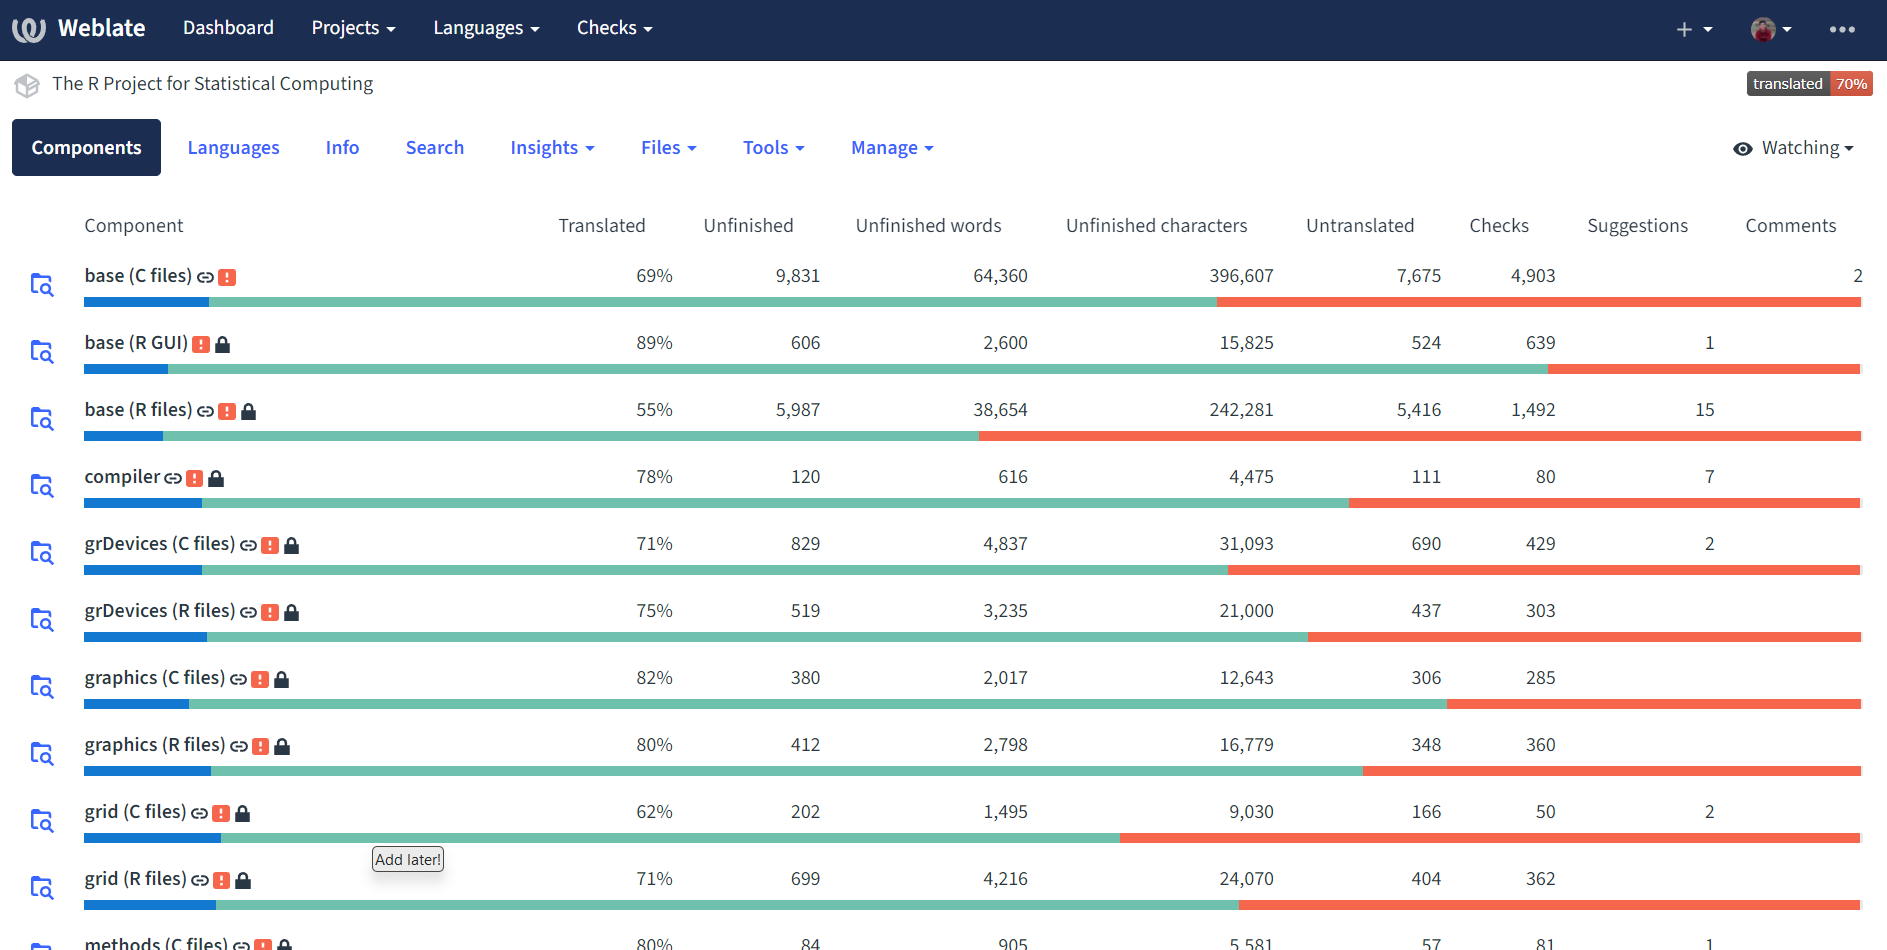
\includegraphics{img/translate_component.png}

\textbf{Step 3: Translate the Message}

Now, you can click on Translate button on your right.

\begin{quote}
Note: More information for String status visit:
\url{https://docs.weblate.org/en/latest/workflows.html\#translation-states}
\end{quote}

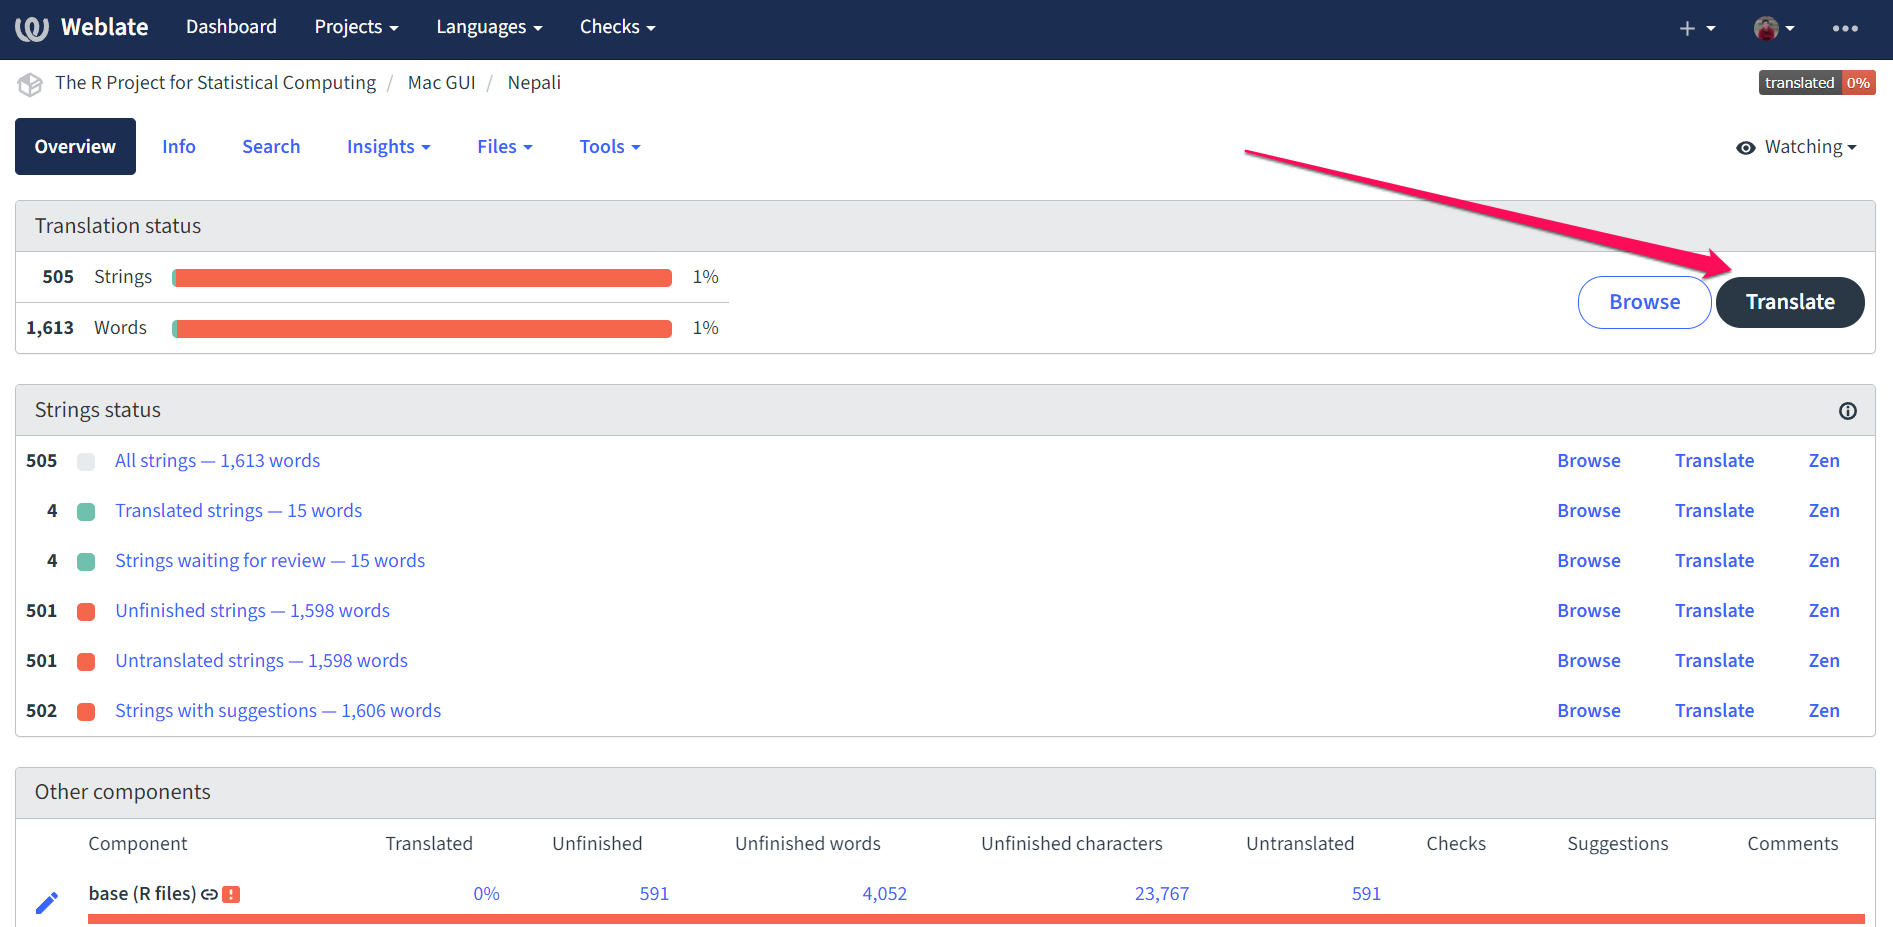
\includegraphics{img/translate_button.png}

Then, start translating the message by typing the translation in the
text box.

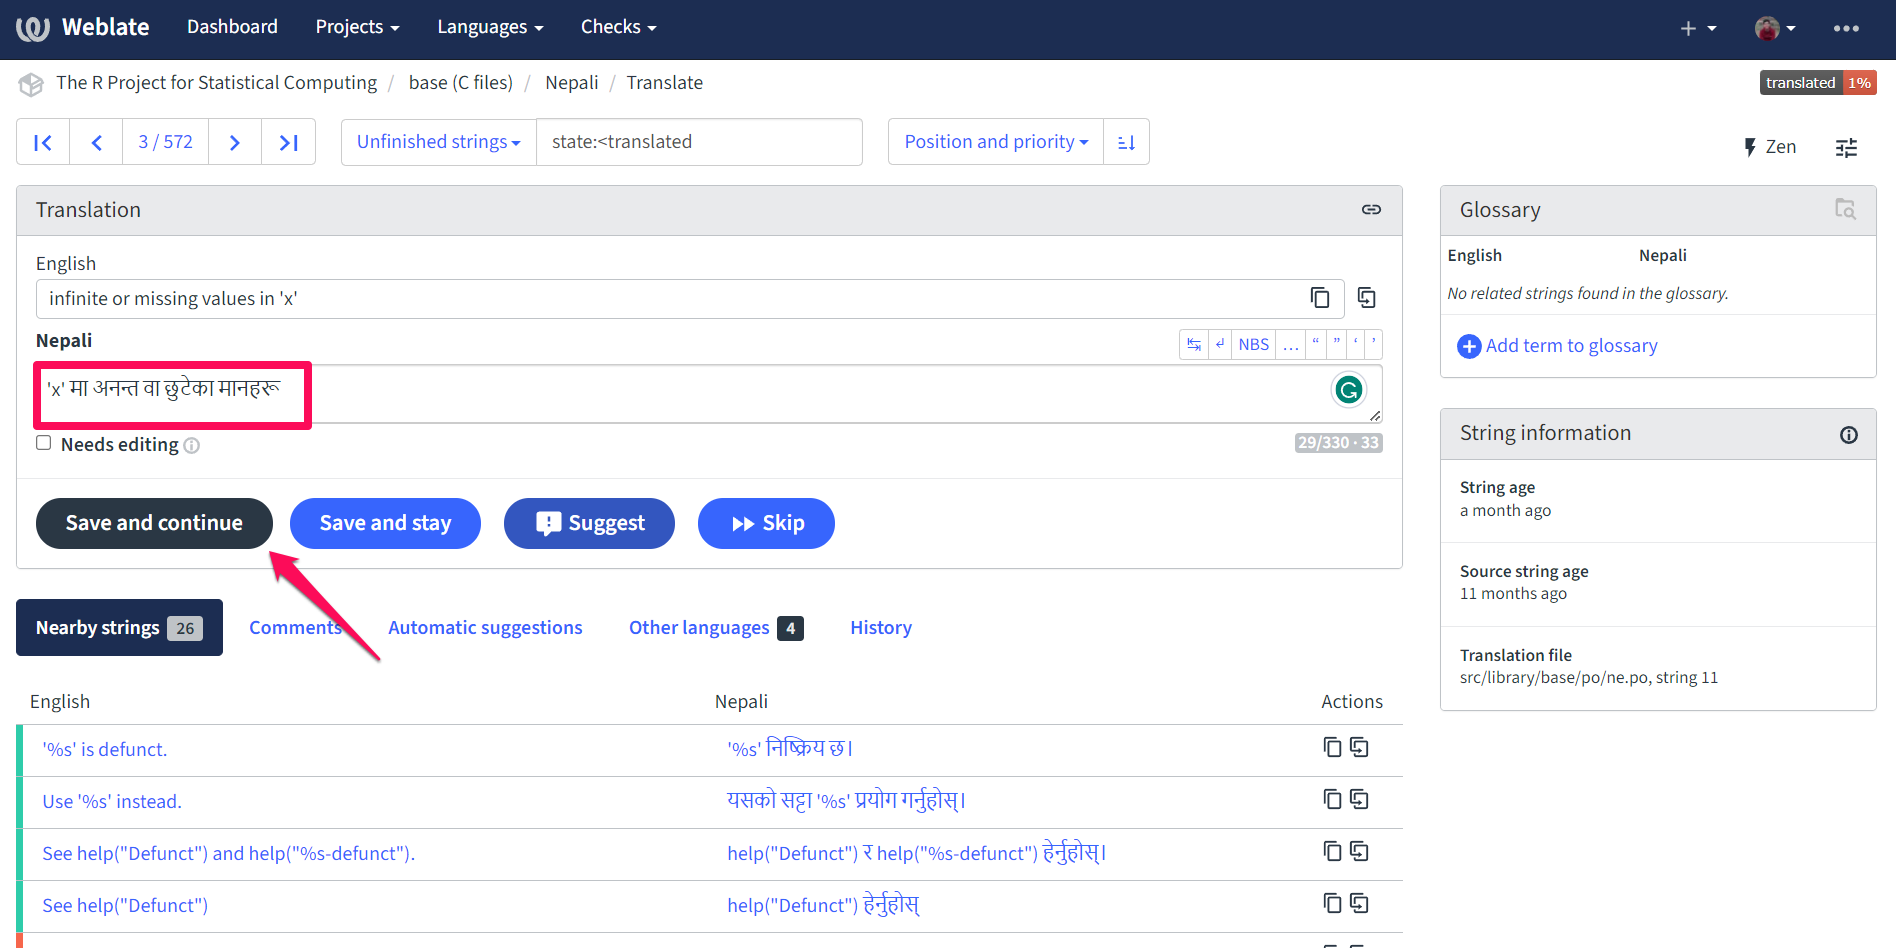
\includegraphics{img/translate_string_and_save.png}

\begin{itemize}
\item
  If you are \textbf{confident} that the \textbf{translation is correct}, make
  sure the ``Needs editing'' box is \textbf{unchecked}.
\item
  If you are \textbf{unsure} about how to translate, write the translation
  as a \textbf{Suggest} button instead.
\item
  Finally, Click \textbf{``Save and Continue''} to save the translation and
  continue.
\end{itemize}

\begin{center}\rule{0.5\linewidth}{0.5pt}\end{center}

\begin{quote}
\textbf{Note:} Use Glossary feature within Weblate making translation easy
and consistent:
\url{https://translate.rx.studio/projects/r-project/glossary/}
\end{quote}

\begin{quote}
\textbf{Note:} Make sure to use Automatic Suggestions as a starting point.
\end{quote}

\begin{enumerate}
\def\labelenumi{\arabic{enumi}.}
\item
  Click on Automatic Suggestions (machine translation)
\item
  Accept it if you think the automatic suggestion looks good
\end{enumerate}

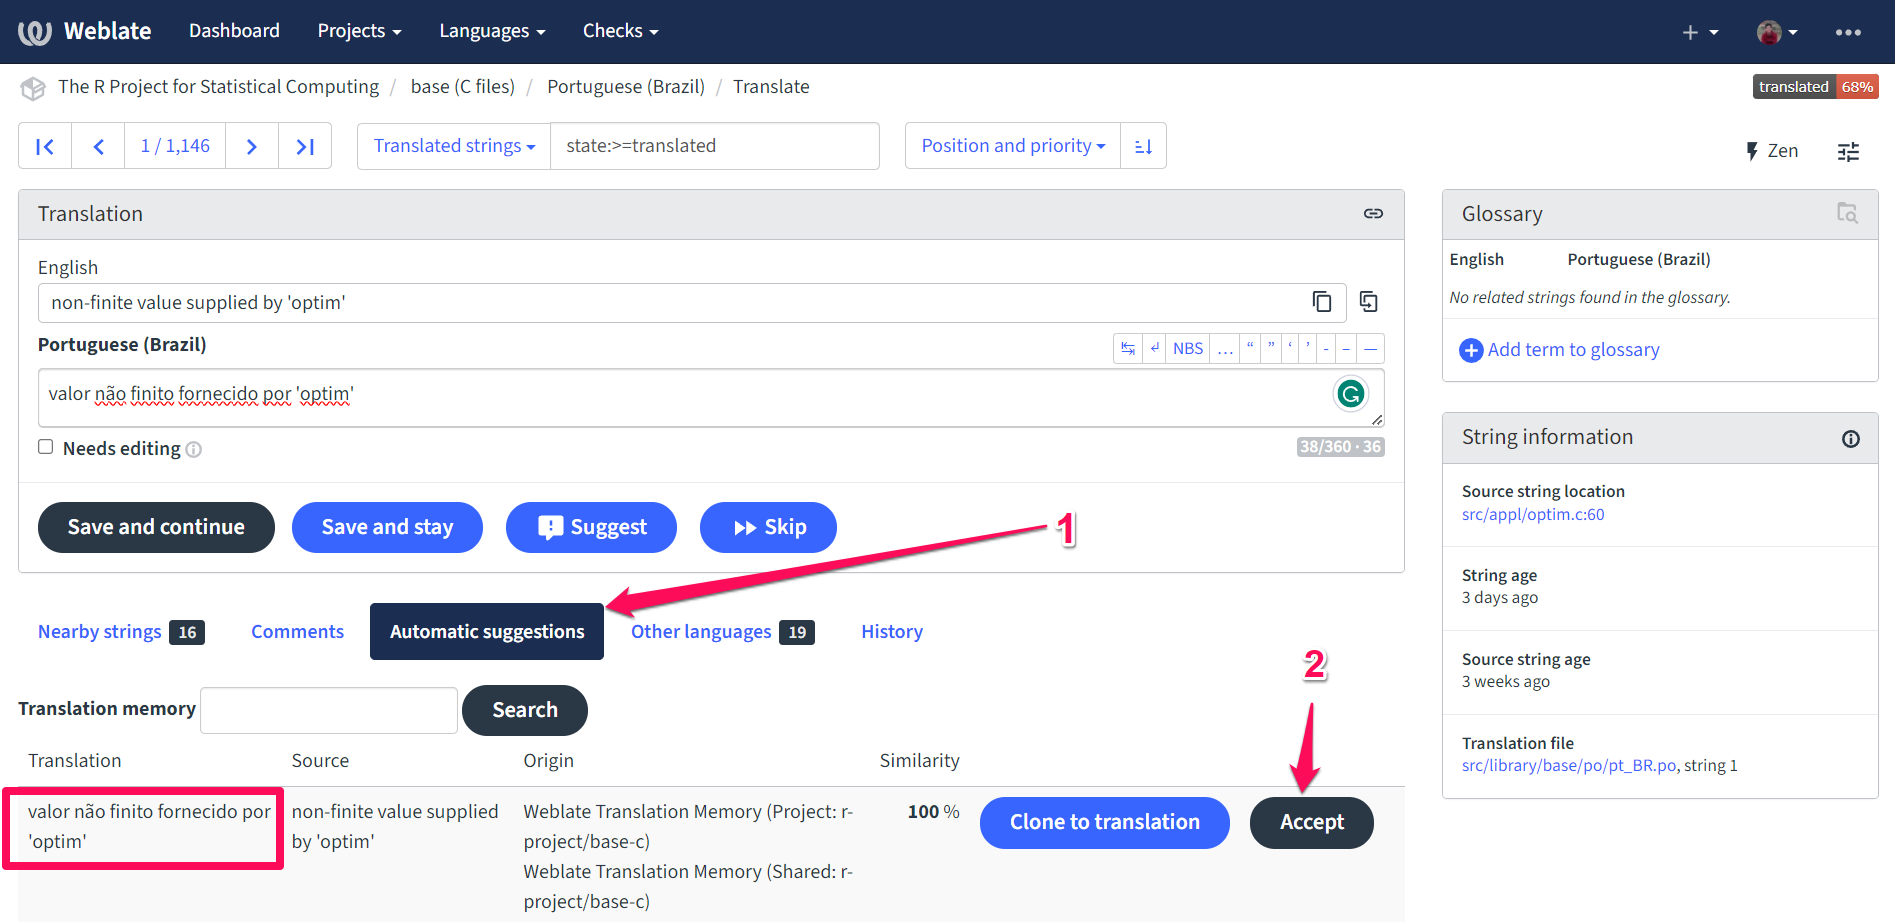
\includegraphics{img/auto-suggestion.png}

\begin{center}\rule{0.5\linewidth}{0.5pt}\end{center}

\textbf{Some Tips to follow:}

\begin{itemize}
\item
  \textbf{Be consistent:} Use the same words and phrases throughout the
  translation to make it consistent and avoid confusion.
\item
  \textbf{Check for technical issues:} After finishing the translation,
  check if you have any alerts or warning in the Weblate string
  status, e.g.~double instead of single space.
\item
  \textbf{Follow language specific guidelines:} Check how other languages
  have translated the string. Even if you are not fluent in another
  language it can give you an idea of how other translators have
  handled it, especially which parts are left verbatim. A detailed
  guide is given here :
  \href{https://contributor.r-project.org/translations/Conventions_for_Languages/\#languages-and-contributions}{Conventions-for-translations\#languages-and-contributions}
\end{itemize}

Related links:
\url{https://contributor.r-project.org/tutorials/translating-r-to-your-language/}

\section{Current status of translations in R}\label{current-status-of-translations-in-r}

\url{https://contributor.r-project.org/translations-dashboard/}

\section{Helpful references}\label{helpful-references}

\begin{itemize}
\tightlist
\item
  Statistical terms glossary
\end{itemize}

\chapter{Testing Pre-release R Versions}\label{TestRVer}

This chapter is inspired from the blog on \href{https://blog.r-project.org/2021/04/28/r-can-use-your-help-testing-r-before-release/index.html}{testing R before release} and discusses how you can help with testing of pre-release versions of R.

\section{Where to test?}\label{where-to-test}

Whenever possible use a fresh package library for testing, even better would be to use \hyperref[VM]{virtual machines} for the testing. This would ensure that you do not damage your existing R installation.

\subsection{Virtual machine}\label{VM}

A free Windows 10 virtual machine is provided by Microsoft (with a 90-day limit) for building, testing, and checking R packages and R itself. Package maintainers who work on Linux and MacOS can use it to test their packages on Windows. Read the \href{https://svn.r-project.org/R-dev-web/trunk/WindowsBuilds/winutf8/ucrt3/vm.html}{instructions} on how to automatically set up the machine to check R packages. Tomas Kalibera describes the details of using virtual machine in the blog \href{https://blog.r-project.org/2021/03/18/virtual-windows-machine-for-checking-r-packages/index.html}{Virtual Windows machine for checking R packages}.

\section{What can you test?}\label{what-can-you-test}

You can test:

\begin{itemize}
\item
  Your own programs.
\item
  Your own workflows.
\item
  Your special ways of installing or setting up R.
\item
  Things that interact with external libraries.
\item
  Interactive R packages.
\end{itemize}

Details of performing testing on various operating systems:

\begin{itemize}
\item
  \href{https://blog.r-project.org/2021/04/28/r-can-use-your-help-testing-r-before-release/index.html\#on-windows}{Windows}
\item
  \href{https://blog.r-project.org/2021/04/28/r-can-use-your-help-testing-r-before-release/index.html\#on-macos}{macOS}
\item
  \href{https://blog.r-project.org/2021/04/28/r-can-use-your-help-testing-r-before-release/index.html\#on-linux}{Linux}
\item
  \href{https://blog.r-project.org/2021/04/28/r-can-use-your-help-testing-r-before-release/index.html\#on-solaris}{Solaris}
\end{itemize}

\section{Writing tests for R}\label{writing-tests-for-r}

Writing tests for R is much like writing tests for your own code. Tests need to be thorough, fast, isolated, consistently repeatable, and as simple as possible.

When you are adding tests to an existing test file, it is also recommended that you study the other tests in that file; it will teach you which precautions you have to take to make your tests robust and portable. We try to have tests both for normal behaviour and for error conditions. Tests live in the \texttt{tests} directory.

\section{Benchmarks}\label{benchmarks}

Benchmarking is useful to test that a change does not degrade performance.

\chapter{R Core Developers}\label{CoreDev}

This page lists the former and current members of the R Core team who have write access to the R source.

\begin{itemize}
\tightlist
\item
  Brian Ripley (present)
\item
  Deepayan Sarkar (present)
\item
  Douglas Bates (present)
\item
  Duncan Murdoch (up to September 2017)
\item
  Duncan Temple Lang (present)
\item
  Friedrich Leisch (present)
\item
  Guido Masarotto (up to June 2003)
\item
  Heiner Schwarte (up to October 1999)
\item
  John Chambers (present)
\item
  Kurt Hornik (present)
\item
  Luke Tierney (present)
\item
  Martin Maechler (present)
\item
  Sebastian Meyer (present)
\item
  Martin Morgan (up to June 2021)
\item
  Martyn Plummer (present)
\item
  Michael Lawrence (present)
\item
  Paul Murrell (present)
\item
  Peter Dalgaard (present)
\item
  Robert Gentleman (present)
\item
  Ross Ihaka (present)
\item
  Seth Falcon (up to August 2015)
\item
  Simon Urbanek (present)
\item
  Stefano lacus (up to July 2014)
\item
  Thomas Lumley (present)
\item
  Tomas Kalibera (present)
\item
  Uwe Ligges (present)
\end{itemize}

View the \href{}{affiliations of R Core members}. We've left it up to the individual core developers to list areas of expertise (or things they are willing to maintain) if they wish.

The \href{https://www.r-project.org/contributors.html}{Contributors page on the R Project website} also lists contributors, outside the R Core team, who provided invaluable help by donating code, bug fixes, and documentation.

\chapter{Where to Get Help}\label{WhereToGetHelp}

If you are working on R it is possible that you will come across an issue where you would need some assistance to solve it. If you require help, there are options available to seek assistance or get some feedback which are discussed in this chapter. If the question involves process or tool usage then please check the rest of this guide first as it should answer your question. Please make sure to search the documentation and resources to see if your question has already been addressed. If not, then ask for assistance in the appropriate forum. Many developers are volunteers and please be polite, patient, and thoughtful when requesting for feedback or help.

\section{Slack}\label{slack}

You can discuss issues related to the development of R and learn about the process of contributing to R on the \href{https://r-contributors.slack.com/}{R Contributors slack}. There are a number of experienced developers on this slack who can answer questions and/or provide feedback. The following channels are available on the R-devel slack for help and feedback with specific areas:

\begin{itemize}
\item
  \#bugreports-for-review: Share bug reports for review/feedback before submitting to Bugzilla.
\item
  \#core-dev-help: Getting help on anything related to R Core contribution.
\item
  \#core-documentation: Discuss patches/improvements to R's documentation.
\item
  \#core-translation: Discuss translating R messages, warnings, and errors into non-English languages.
\item
  \#patches-for-review: Share patches for peer review before submitting to R Core.
\end{itemize}

Note: You may not be able to access the history of these channels, so it cannot be used as a knowledge base of sorts.

\section{Mailing lists}\label{mailing-lists}

There are quite a few \href{https://www.r-project.org/mail.html}{mailing lists} for getting help with R:

\begin{itemize}
\tightlist
\item
  \href{https://stat.ethz.ch/mailman/listinfo/r-devel}{R-devel}:

  \begin{itemize}
  \tightlist
  \item
    Questions and discussion about development \emph{of} R vs.~\emph{with} R.
  \item
    Getting help with technical programming issues, e.g.~interfacing R with C/C++.
  \item
    Proposals of new functionality for R.
  \item
    Pre-testing of new versions of R.
  \item
    Enhancements and patches to the R source code and the R documentation.
  \item
    Posting examples and benchmarks.
  \end{itemize}
\item
  \href{https://stat.ethz.ch/mailman/listinfo/r-help}{R-help}:

  \begin{itemize}
  \tightlist
  \item
    Discussions about problems and solutions using R.
  \end{itemize}
\item
  \href{https://stat.ethz.ch/mailman/listinfo/r-package-devel}{R-package-devel}:

  \begin{itemize}
  \tightlist
  \item
    Getting help about package development in R.
  \item
    Learning about the package development process.
  \item
    Discussing problems developing a package (or problem in passing the R CMD check).
  \end{itemize}
\end{itemize}

Please avoid cross-posting to both the R-package-devel and the R-devel mailing lists.

\section{File a bug}\label{file-a-bug}

If you strongly suspect you have come across a bug (be it in the build process, or in other areas), then \hyperref[ReportBug]{report it on Bugzilla}.

\chapter{News and Announcements}\label{News}

Here are some resources that can be useful to keep up with the developments in R:

\section{Blogs}\label{blogs}

The \href{https://www.r-project.org/}{R project} maintains \href{https://blog.r-project.org/}{The R Blog} with posts mainly written by the R Core Team. News of changes in the development version of R found on the \href{https://developer.r-project.org/blosxom.cgi/R-devel}{Daily News about R-devel} blog which is updated daily.

\section{Conferences}\label{conferences}

Updates about conferences actively supported or endorsed by The R Foundation can be found \href{https://www.r-project.org/conferences/}{here}. These conferences are organised by members from the R community.

\section{Journal}\label{journal}

\href{https://journal.r-project.org/}{The R Journal} is an open access and refereed journal featuring short to medium length articles that should be of interest to users or developers of R. It also has a news section where information on, changes in R (new features of the latest release), changes on CRAN (new add-on packages, manuals, binary contributions, mirrors, etc.), upcoming conferences, and conference reports is provided.

\section{Mailing lists}\label{mailing-lists-1}

\begin{itemize}
\tightlist
\item
  \href{https://stat.ethz.ch/mailman/listinfo/r-announce}{R-announce}: A moderated mailing list used for announcements by the R Core Development Team. Major announcements about the development of R and the availability of new code are made here.
\item
  \href{https://stat.ethz.ch/mailman/listinfo/r-packages}{R-packages}: A moderated mailing list for announcements about contributed R packages (typically on \href{https://cran.r-project.org/}{CRAN}) and similar R project extensions.
\end{itemize}

\section{Twitter}\label{twitter}

Follow \href{https://twitter.com/R_dev_news}{@R\_dev\_news} on Twitter for news of \href{https://developer.r-project.org/RSSfeeds.html}{changes in the development version of R} and new posts on \href{https://blog.r-project.org/}{The R Blog} announcements.

\chapter{Developer Tools}\label{DevTools}

This chapter lists resources and tools which R developers may use. Here we will go over some commonly used tools that are relevant to R's workflow. As there are several ways to accomplish these tasks, this chapter reflects methods suitable for new contributors. Experienced contributors may desire a different approach.

\section{Subversion (svn) client}\label{subversion-svn-client}

Subversion (svn) is a version control system that tracks any changes made to files and directories. You can install either the TortoiseSVN (\url{https://tortoisesvn.net/}, command line tool, and Windows Explorer integration) or the SlikSVN (\url{https://sliksvn.com/download/}, just the command line tool) client. They have Windows installers and can be used from Windows cmd or RStudio terminal.

Some resources for learning subversion commands:

\begin{enumerate}
\def\labelenumi{\arabic{enumi}.}
\item
  \href{http://subversion.apache.org/quick-start}{Apache Subversion quick start guide}
\item
  \href{https://tortoisesvn.net/docs/nightly/TortoiseSVN_en/tsvn-cli-main.html}{TortoiseSVN commands}
\item
  \href{https://sliksvn.com/support/subversion-basics-using-check-out-update-check-in-commit/}{SlikSVN basics}
\item
  \href{http://svnbook.red-bean.com/}{Subversion book}
\end{enumerate}

\section{Globally search for a regular expression and print matching lines (grep)}\label{globally-search-for-a-regular-expression-and-print-matching-lines-grep}

\href{https://en.wikipedia.org/wiki/Grep}{grep} is a command line utility for searching plain text data sets for lines that match a regular expression. Refer the \href{https://www.gnu.org/software/grep/manual/grep.html}{grep manual} for more commands.

\section{Git}\label{git}

\href{https://en.wikipedia.org/wiki/Git}{Git} is also a version control system for tracking changes in any files and directories. View \href{https://git-scm.com/doc}{git documentation} for learning git commands.

\section{GitHub}\label{github}

Some resources that are useful while using GitHub are:

\begin{enumerate}
\def\labelenumi{\arabic{enumi}.}
\item
  \href{https://docs.github.com/en/github/collaborating-with-issues-and-pull-requests/creating-a-pull-request}{Creating a pull request}
\item
  \href{https://docs.github.com/en/github/managing-your-work-on-github/opening-an-issue-from-code}{Opening an issue from code}
\item
  \href{https://docs.github.com/en/github/collaborating-with-issues-and-pull-requests/resolving-a-merge-conflict-on-github}{Resolving a merge conflict on GitHub}
\end{enumerate}

  \bibliography{book.bib}

\end{document}
